\chapter{Results: \deploy Demonstration}
In this chapter, we demonstrate \deploy's capabilities
in simple and complex \Cyclus transition scenario simulations.  
This chapter has two sections: 
\begin{enumerate}
    \item \deploy demonstration for simple transition scenarios
    \item \deploy demonstration for the EG01-30 transition scenario
\end{enumerate}

\section{\deploy Demonstration of Simple Transition Scenarios}
\label{sec:demo}

This section demonstrates \deploy's capability 
to effectively set up a simple transition scenario simulation 
for constant, linearly increasing, and 
sinusoidal power demand simulations.
These simulations only include
three facility types: \texttt{source}, \texttt{reactor}, and 
\texttt{sink}. 
The simulations begin with ten \texttt{reactor} facilities 
(\texttt{reactor1} to \texttt{reactor10}). 
These reactors have staggered cycle lengths and lifetimes to prevent 
simultaneous refueling and to set up gradual decommissioning. 
\deploy is configured to deploy \texttt{new reactor} facilities
to meet the loss of power supply created by the decommissioning 
of the initial \texttt{reactor} facilities. 
Table \ref{tab:demonstrations} shows the 
\deploy input parameters for these simulations.
Figure \ref{fig:powerplots} shows the user-defined power demand curves 
for the three simulations that \deploy deploys facilities to meet.

\begin{table}[]
    \caption{\deploy's input parameters for the simple constant, 
    linearly increasing, and sinusoidal power demand 
    transition scenarios.}
    \label{tab:demonstrations}
    \resizebox{1\textwidth}{!}{%
    \doublespacing
    \begin{tabular}{l|c|c|c}
    \hline
    &\multicolumn{3}{c}{\textbf{Simulation Description}}                                                                                                                                                                                                                                                       \\ \hline
    \multicolumn{1}{c|}{\textbf{Input Parameter}}                           & \multicolumn{1}{l|}{\textbf{Constant Power}}                                                                 & \textbf{\begin{tabular}[c]{@{}l@{}}Linearly Increasing \\ Power\end{tabular}}                  & \textbf{Sinusoidal Power}                                                                  \\ \hline
    Demand driving commodity                                       & \multicolumn{3}{c}{Power}                                                                                                                                                                                                                                                                                 \\ \hline 
    Demand equation [MW]                                               & \multicolumn{1}{l|}{10000}                                                                                & \begin{tabular}[c]{@{}l@{}}t\textless 40: 10000\\ t\textgreater{}=40: 250*t\end{tabular} & 10000+ 1000*$\sin(\pi*t/3)$                                                                 \\ \hline 
    Available Facilities                                           & \multicolumn{3}{c}{Source, Reactor, Sink}                                                                                                                                                                                                                                                                 \\ \hline
    Prediction method                                              & \multicolumn{1}{l|}{\begin{tabular}[c]{@{}l@{}}Power: \texttt{FFT}\\ Fuel: \texttt{MA}\\ Spent fuel: \texttt{MA}\end{tabular}}          & \begin{tabular}[c]{@{}l@{}}Power: FFT\\ Fuel: MA\\ Spent fuel: FFT\end{tabular}                & \begin{tabular}[c]{@{}l@{}}Power: HW\\ Fuel: MA\\ Spent fuel: FFT\end{tabular}             \\\hline 
    Deployment Driving Method                                      & \multicolumn{3}{c}{Installed Capacity}                                                                                                                                                                                                                                                                    \\ \hline
    Buffer type                                                    & \multicolumn{3}{c}{Absolute}                                                                                                                                                                                                                                                                              \\ \hline 
    Buffer size                                                    & \multicolumn{1}{l|}{\begin{tabular}[c]{@{}l@{}}Power: 3000 MW\\ Fuel: 0 kg \\ Spent fuel: 0 kg\end{tabular}} & \begin{tabular}[c]{@{}l@{}}Power: 2000 MW\\ Fuel: 1000 kg \\ Spent fuel: 0 kg\end{tabular}     & \begin{tabular}[c]{@{}l@{}}Power: 2000 MW\\ Fuel: 1000 kg \\ Spent fuel: 0 kg\end{tabular} \\ \hline
    \end{tabular}
    }
    \end{table}

    \begin{figure}[]
        \begin{center}
            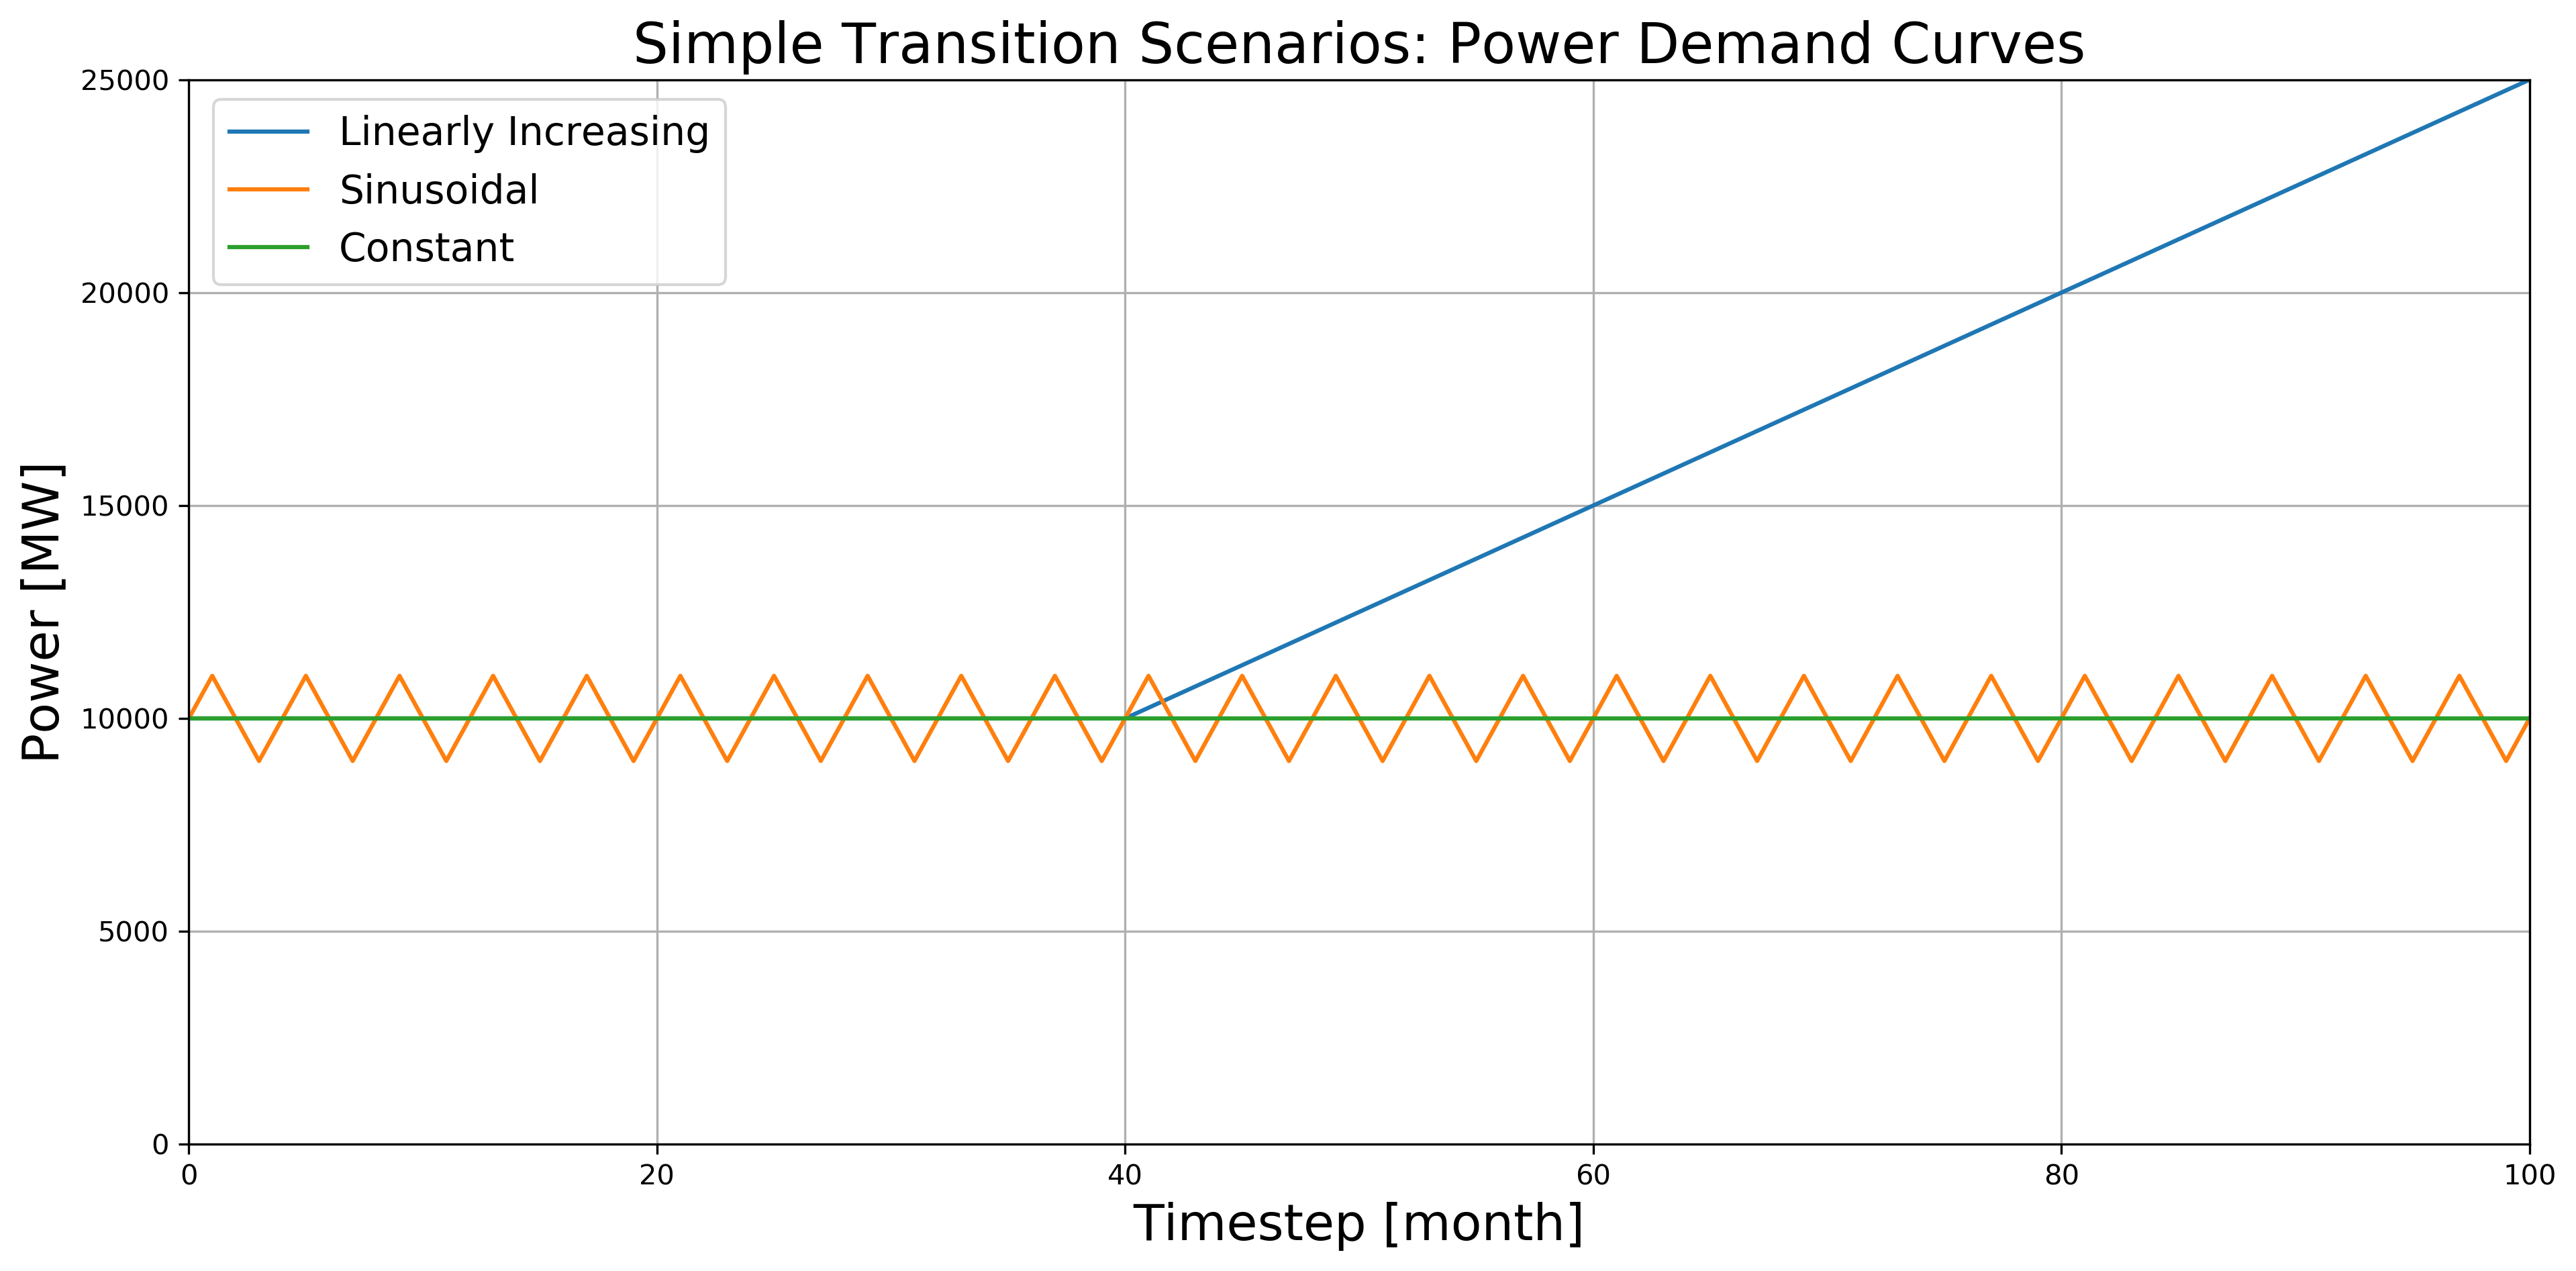
\includegraphics[scale=0.45]{./figures/powerplots.png}
        \end{center}
            \caption{Power demand curves for the simple constant, 
            linearly increasing, and sinusoidal power demand 
            transition scenarios.}
        \label{fig:powerplots}
    \end{figure}

\subsection{Simple Transition Scenario Simulation: Constant Demand}
Figures \ref{fig:constanttransition-power}, \ref{fig:constanttransition-fuel},
and \ref{fig:constanttransition-spentfuel} demonstrate \deploy's capability 
to deploy reactor and supporting facilities to minimize undersupply 
when meeting linearly increasing power demand and subsequent secondary 
commodities demand.  
Table \ref{tab:transition-scenario-results} shows the number of 
undersupplied timesteps. 
In Figure \ref{fig:constanttransition-power}, there exist no time steps 
in which the supply of power falls under demand, meeting the main 
objective of \deploy. 
By using a combination of the \texttt{FFT} method for 
predicting demand and setting the power supply buffer to 3000MW 
(the capacity of 3 reactors), the user minimizes the number of 
undersupplied timesteps for every commodity.

In figure \ref{fig:constanttransition-fuel},
a large-throughput source facility is initially
deployed to meet the large initial fuel demand for the commissioning 
of ten reactors. 
By having a large-throughput source facility exist for the 
first few time steps, \deploy does not deploy supporting
facilities that become redundant at later times in  
the simulation.
This reflects reality in which reactor manufacturers accumulate
an appropriate amount of fuel inventory before starting 
up reactors. 
There is one time step in which a power undersupply exists after the 
decommissioning of the large initial facility; 
this is unavoidable as the prediction methods in \deploy are 
unable to foresee this sudden drop in demand. 

    \begin{figure}[]
        \centering
        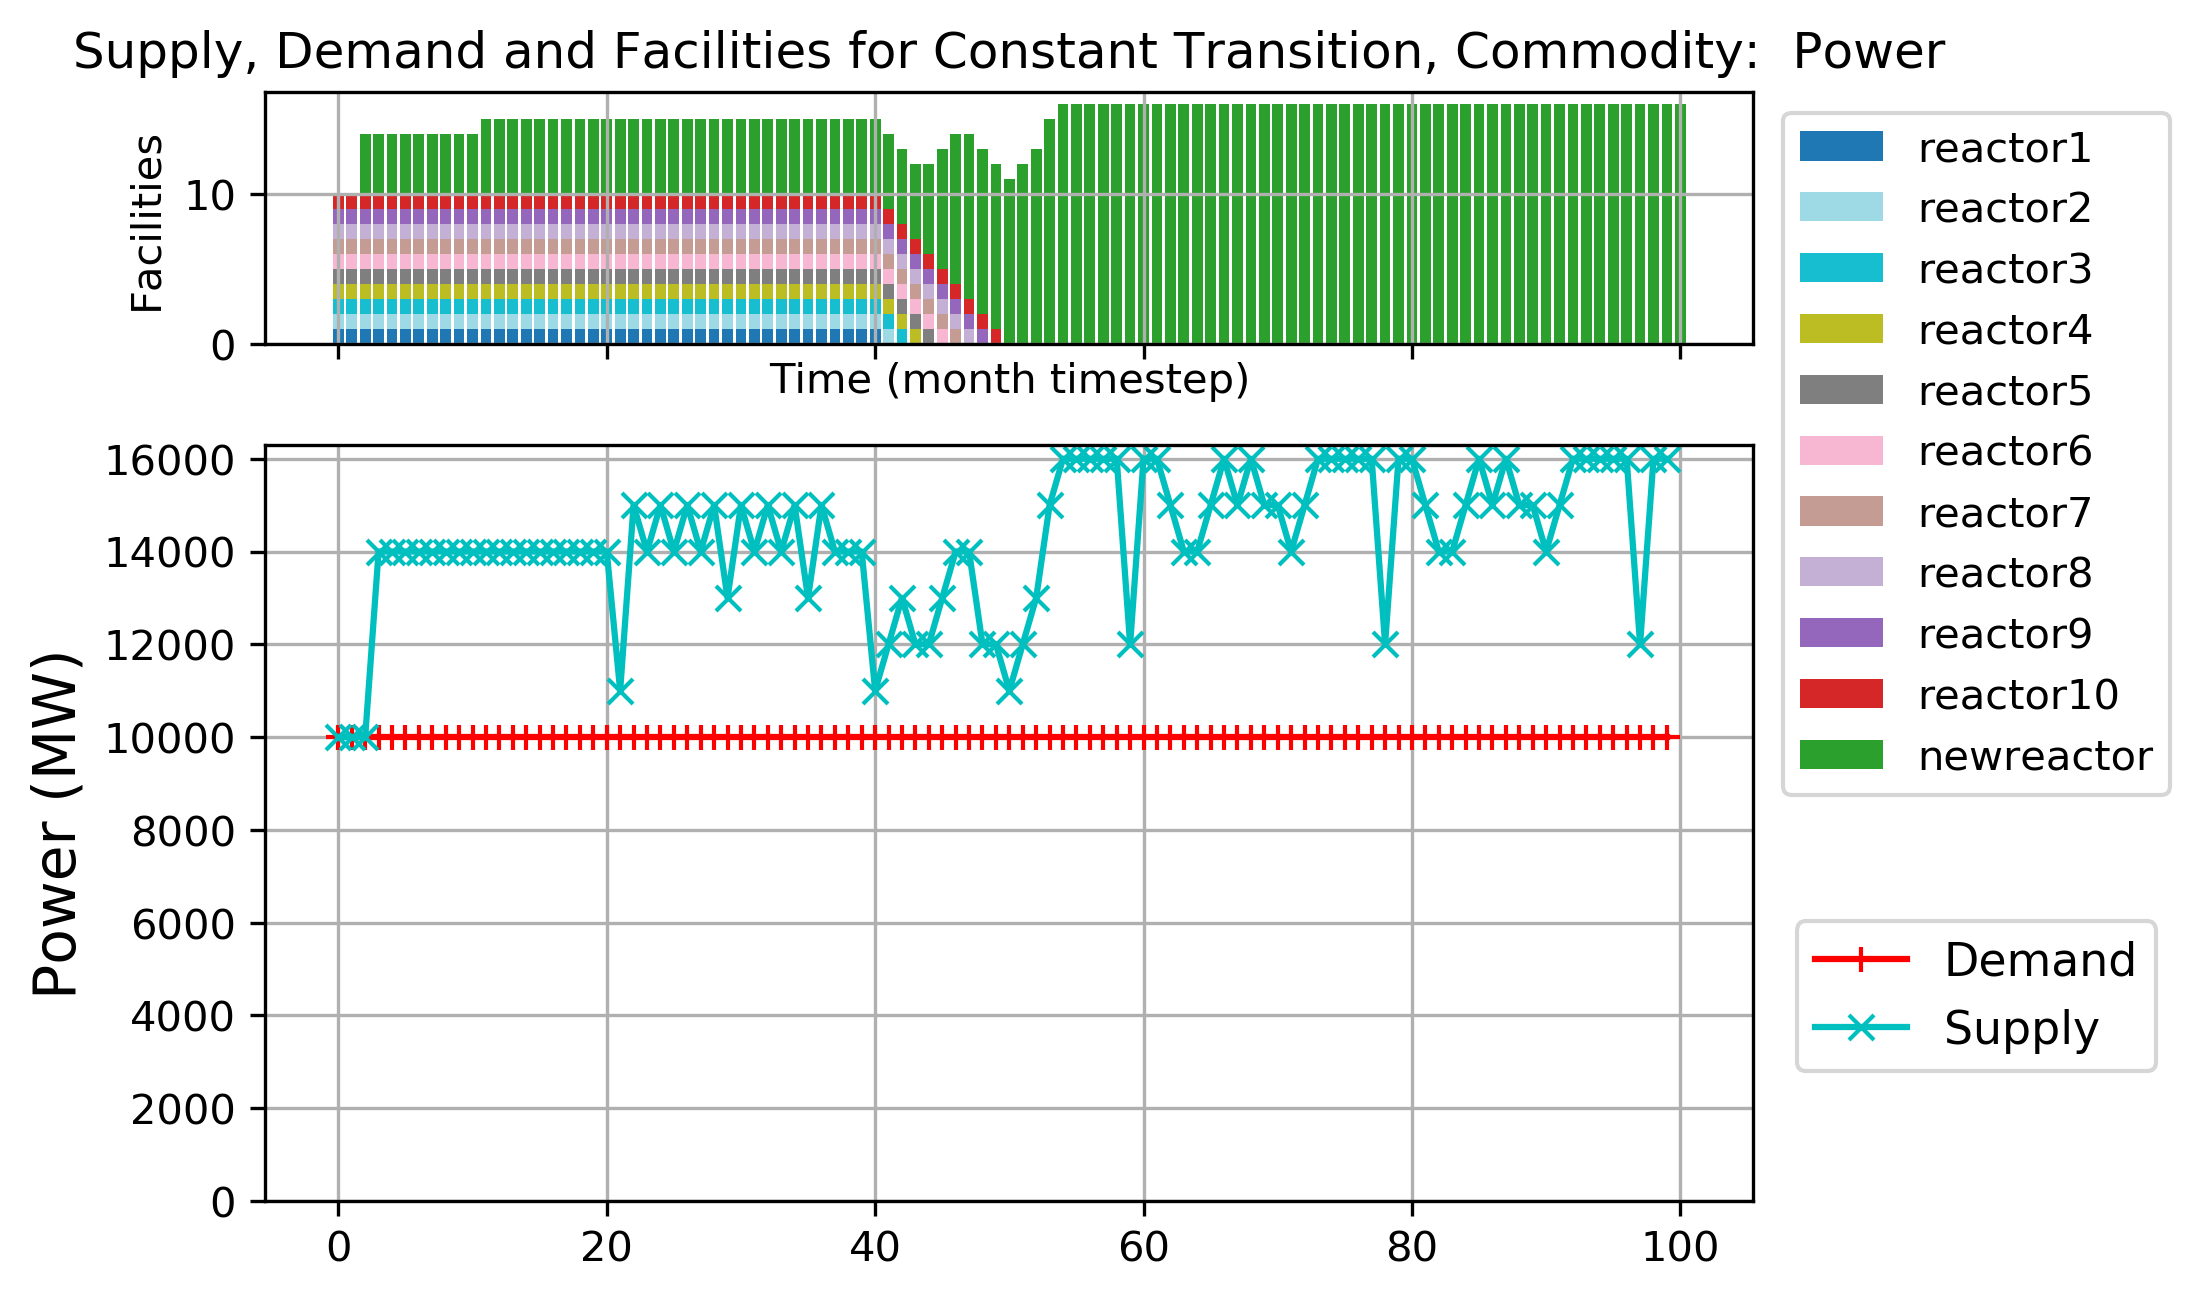
\includegraphics[width=0.9\linewidth]{figures/constanttransition-power.png} 
            \caption{Power demand and supply, and reactor facility deployment plot for  
            a simple constant power demand transition scenario with 
            three facility types: \texttt{source}, \texttt{reactor}, and \texttt{sink}.
            Power demand is a user-defined equation and power is supplied by the reactors.
            There are no time steps with undersupply of power.}
            \label{fig:constanttransition-power}
    \end{figure}

    \begin{figure}[]
        \centering
        \begin{subfigure}[t]{1\textwidth}
            \centering
            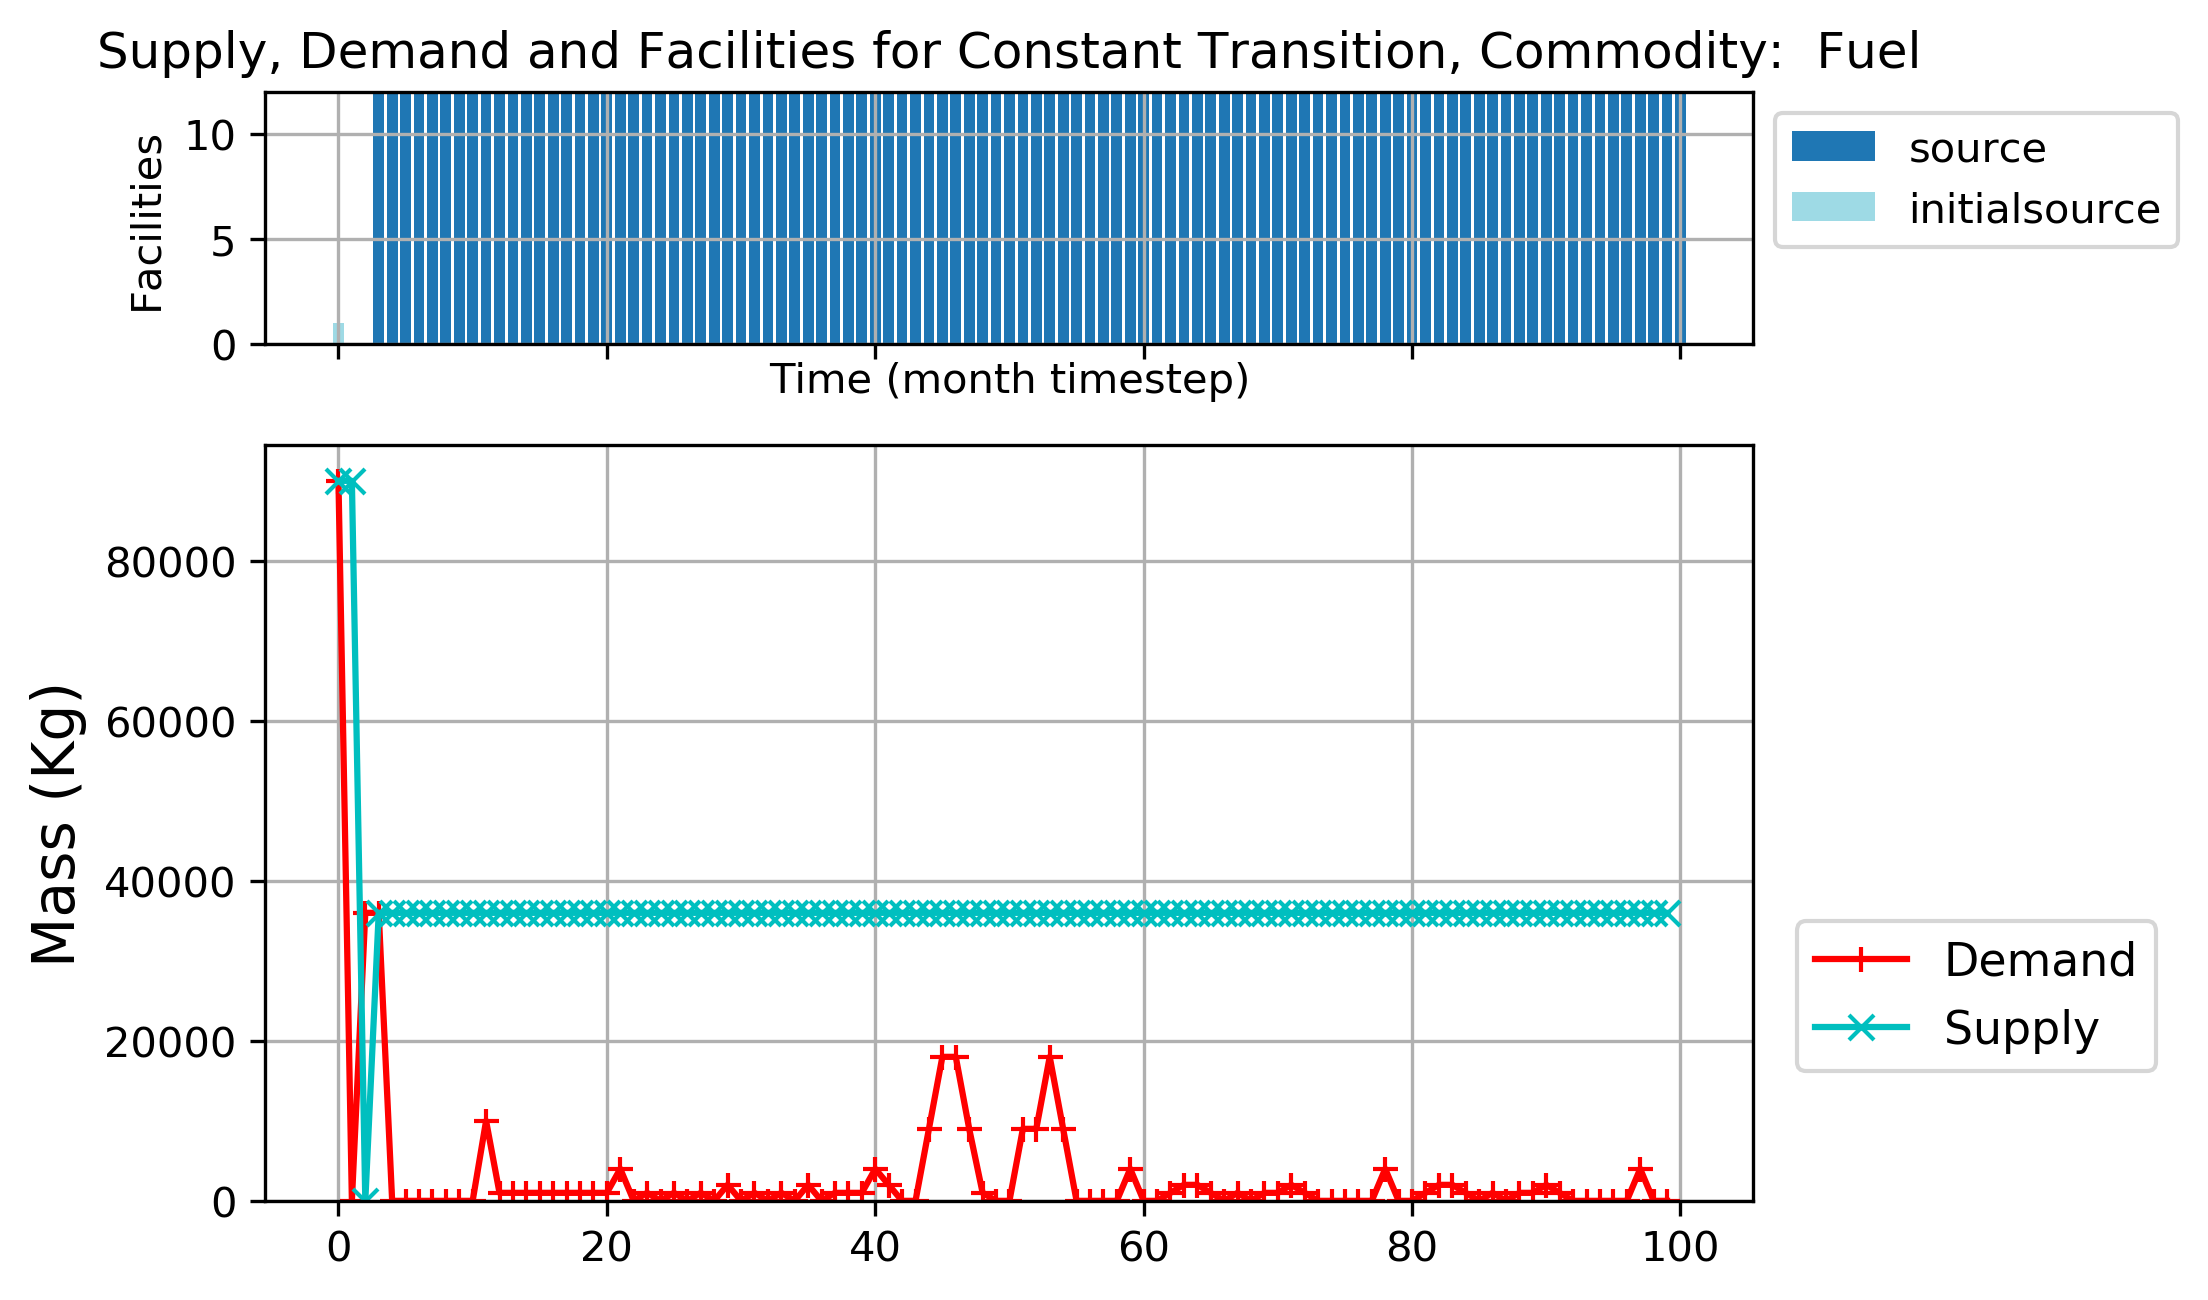
\includegraphics[width=0.9\linewidth]{figures/constanttransition-fuel.png} 
            \caption{Fuel demand and supply, and source facility deployment plot.
            Fuel is demanded by reactors and supplied by source facilities.
            There is only one time step with undersupply of fuel.}
            \label{fig:constanttransition-fuel}
        \end{subfigure}
        \begin{subfigure}[t]{1\textwidth}
            \centering
            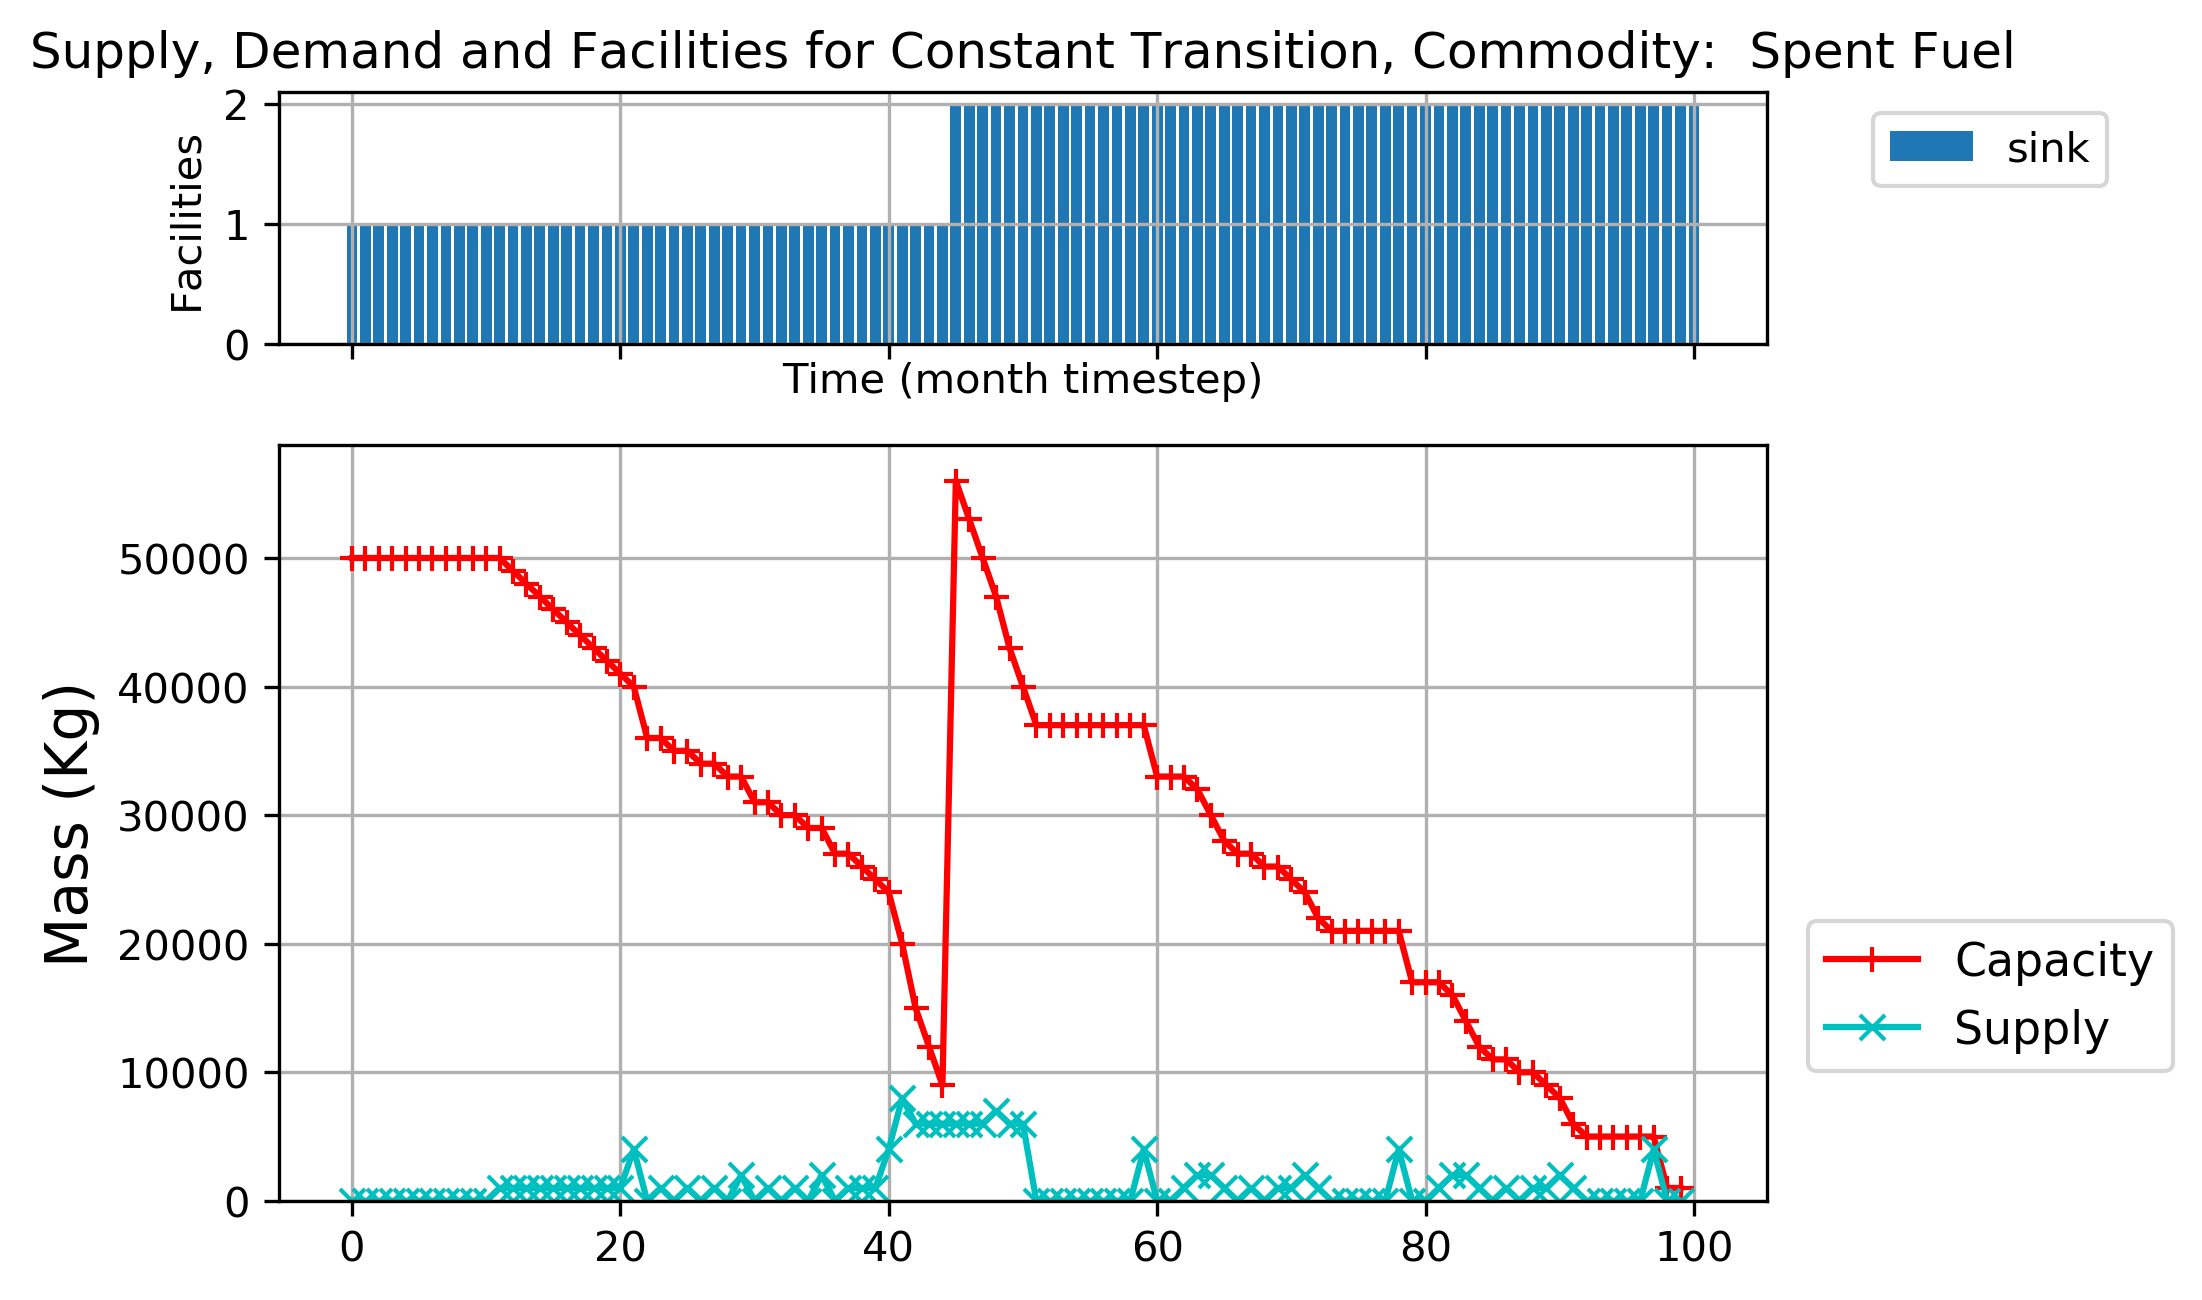
\includegraphics[width=0.9\linewidth]{figures/constanttransition-spentfuel.png} 
            \caption{Spent fuel demand and supply, and sink facility deployment plot.
                Spent Fuel is supplied by reactors and the capacity to store them 
                is provided by sink facilities.
            There are no time steps with under-capacity of sink space.}
            \label{fig:constanttransition-spentfuel}
        \end{subfigure}
        \caption{Simple constant power demand transition scenario with 
        three facility types: \texttt{source}, \texttt{reactor}, and \texttt{sink}.}
    \end{figure}

    \subsection{Simple Transition Scenario Simulation: Linearly Increasing Demand}

    Figures \ref{fig:growingtransition-power}, \ref{fig:growingtransition-fuel},
    and \ref{fig:growingtransition-spentfuel} demonstrate \deploy's capability 
    to deploy reactor and supporting facilities to minimize undersupply 
    when meeting linearly increasing power demand and subsequent secondary 
    commodities demand. 
    This transition utilizes a smaller power supply buffer compared with the constant 
    power transition scenario to minimize power undersupply.
    Table \ref{tab:transition-scenario-results} shows the number of 
    undersupplied timesteps. 
    In Figure \ref{fig:growingtransition-power}, there exist no time steps 
    in which the supply of power falls under demand, meeting the main 
    objective of \deploy. 
    
    \begin{figure}[]
        \centering
        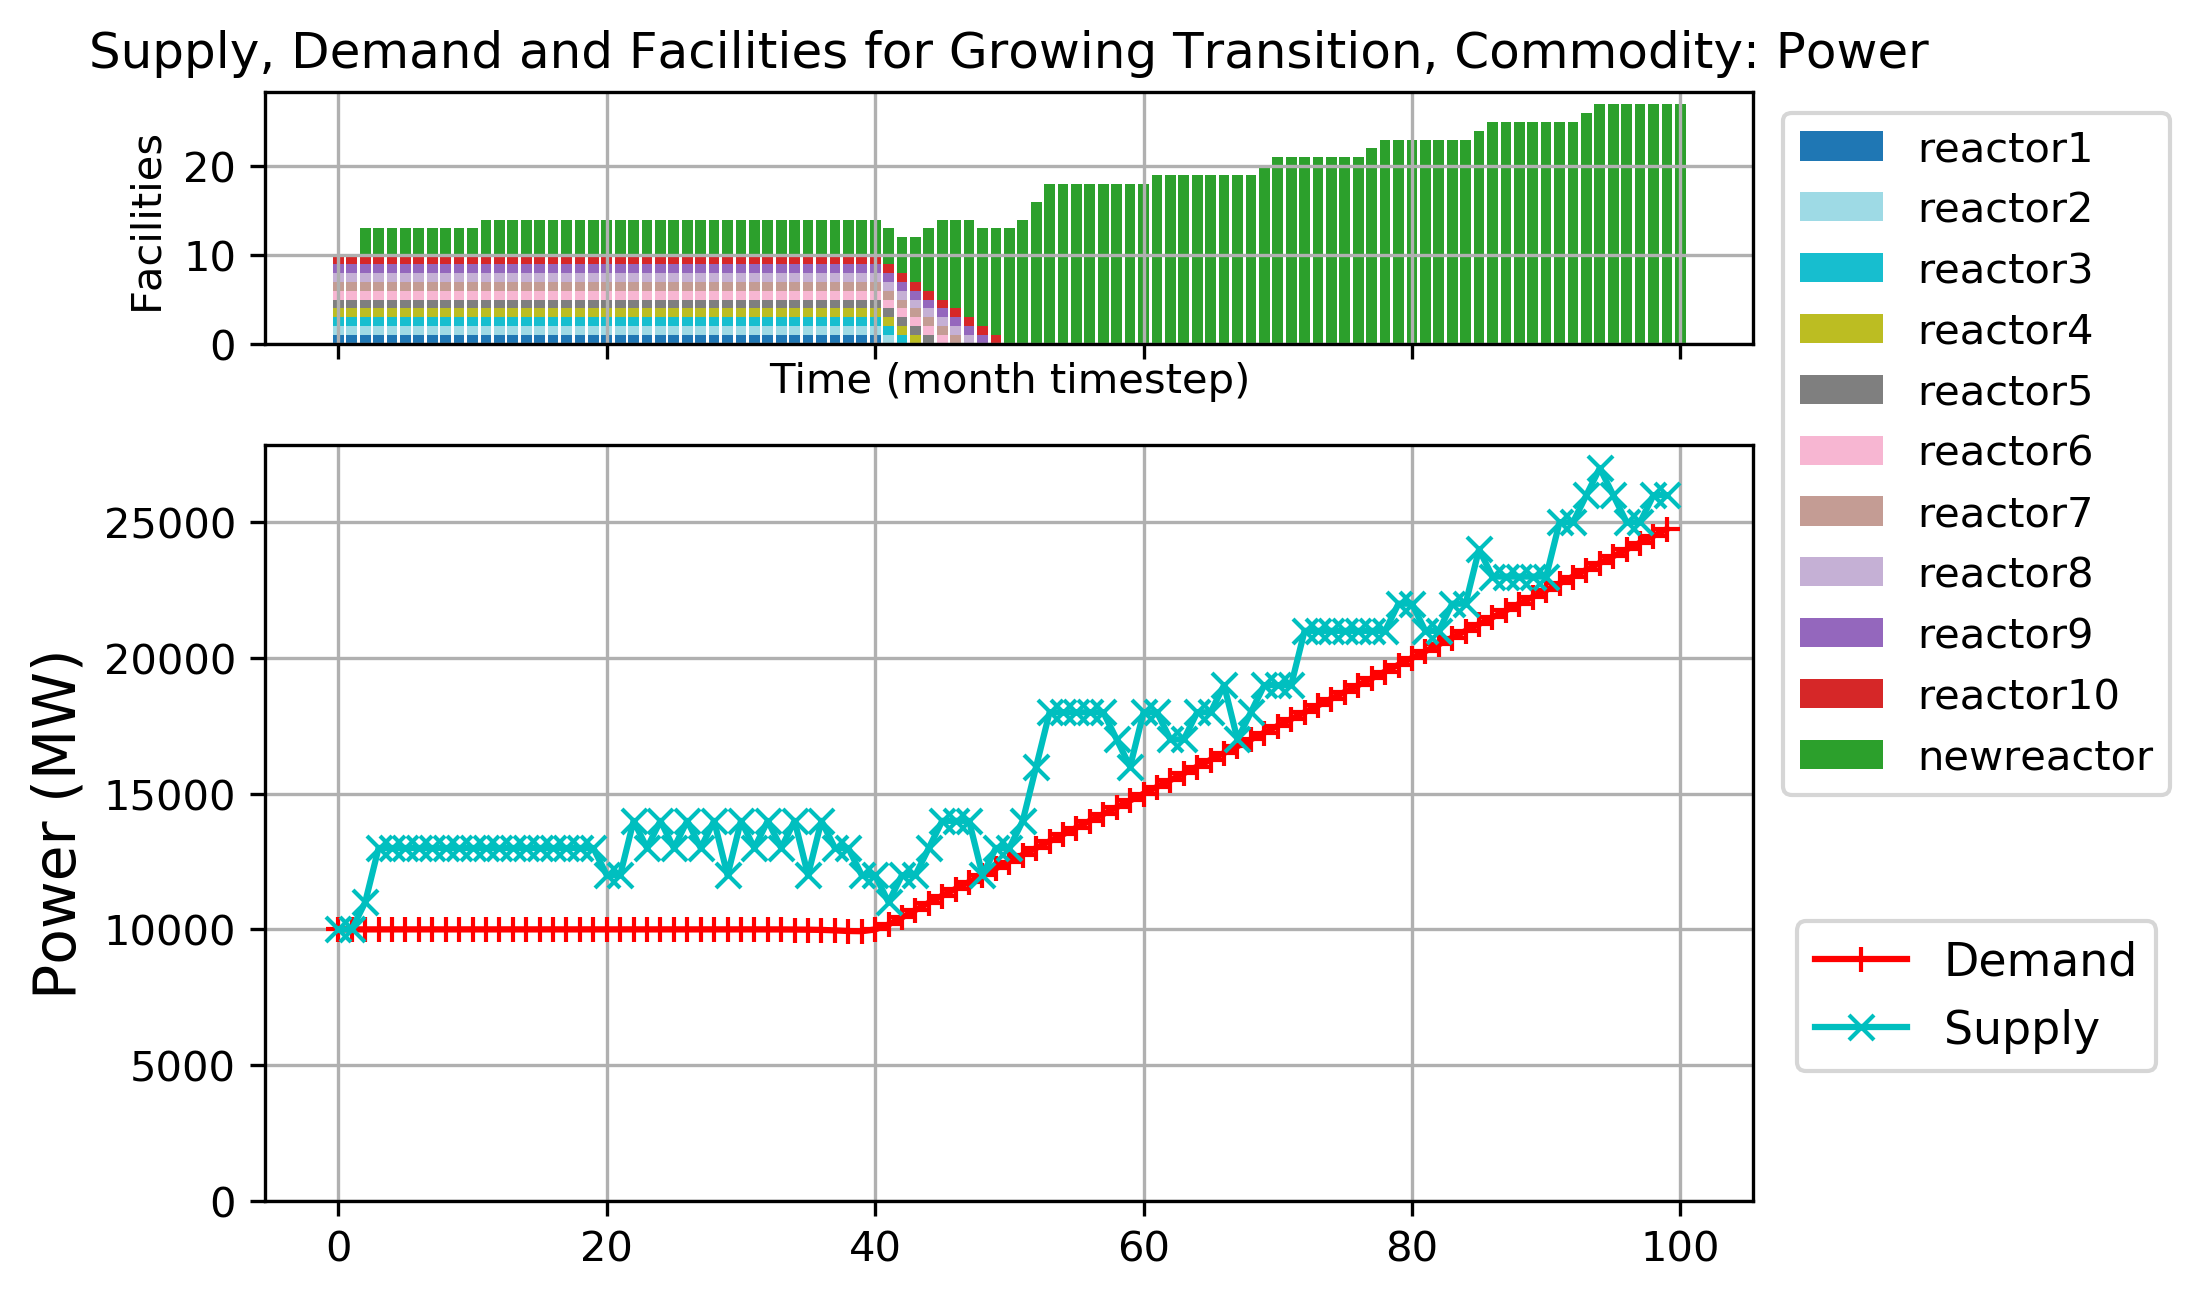
\includegraphics[width=0.9\linewidth]{figures/growingtransition-power.png} 
            \caption{Power demand and supply, and reactor facility deployment plot for  
            a simple linearly increasing power demand transition scenario with 
            three facility types: \texttt{source}, \texttt{reactor}, and \texttt{sink}.
            Power demand is a user-defined equation and power is supplied by the reactors.
            There are no time steps with undersupply of power.}
            \label{fig:growingtransition-power}
    \end{figure}
    
    \begin{figure}[]
        \centering
        \begin{subfigure}[t]{\textwidth}
            \centering
            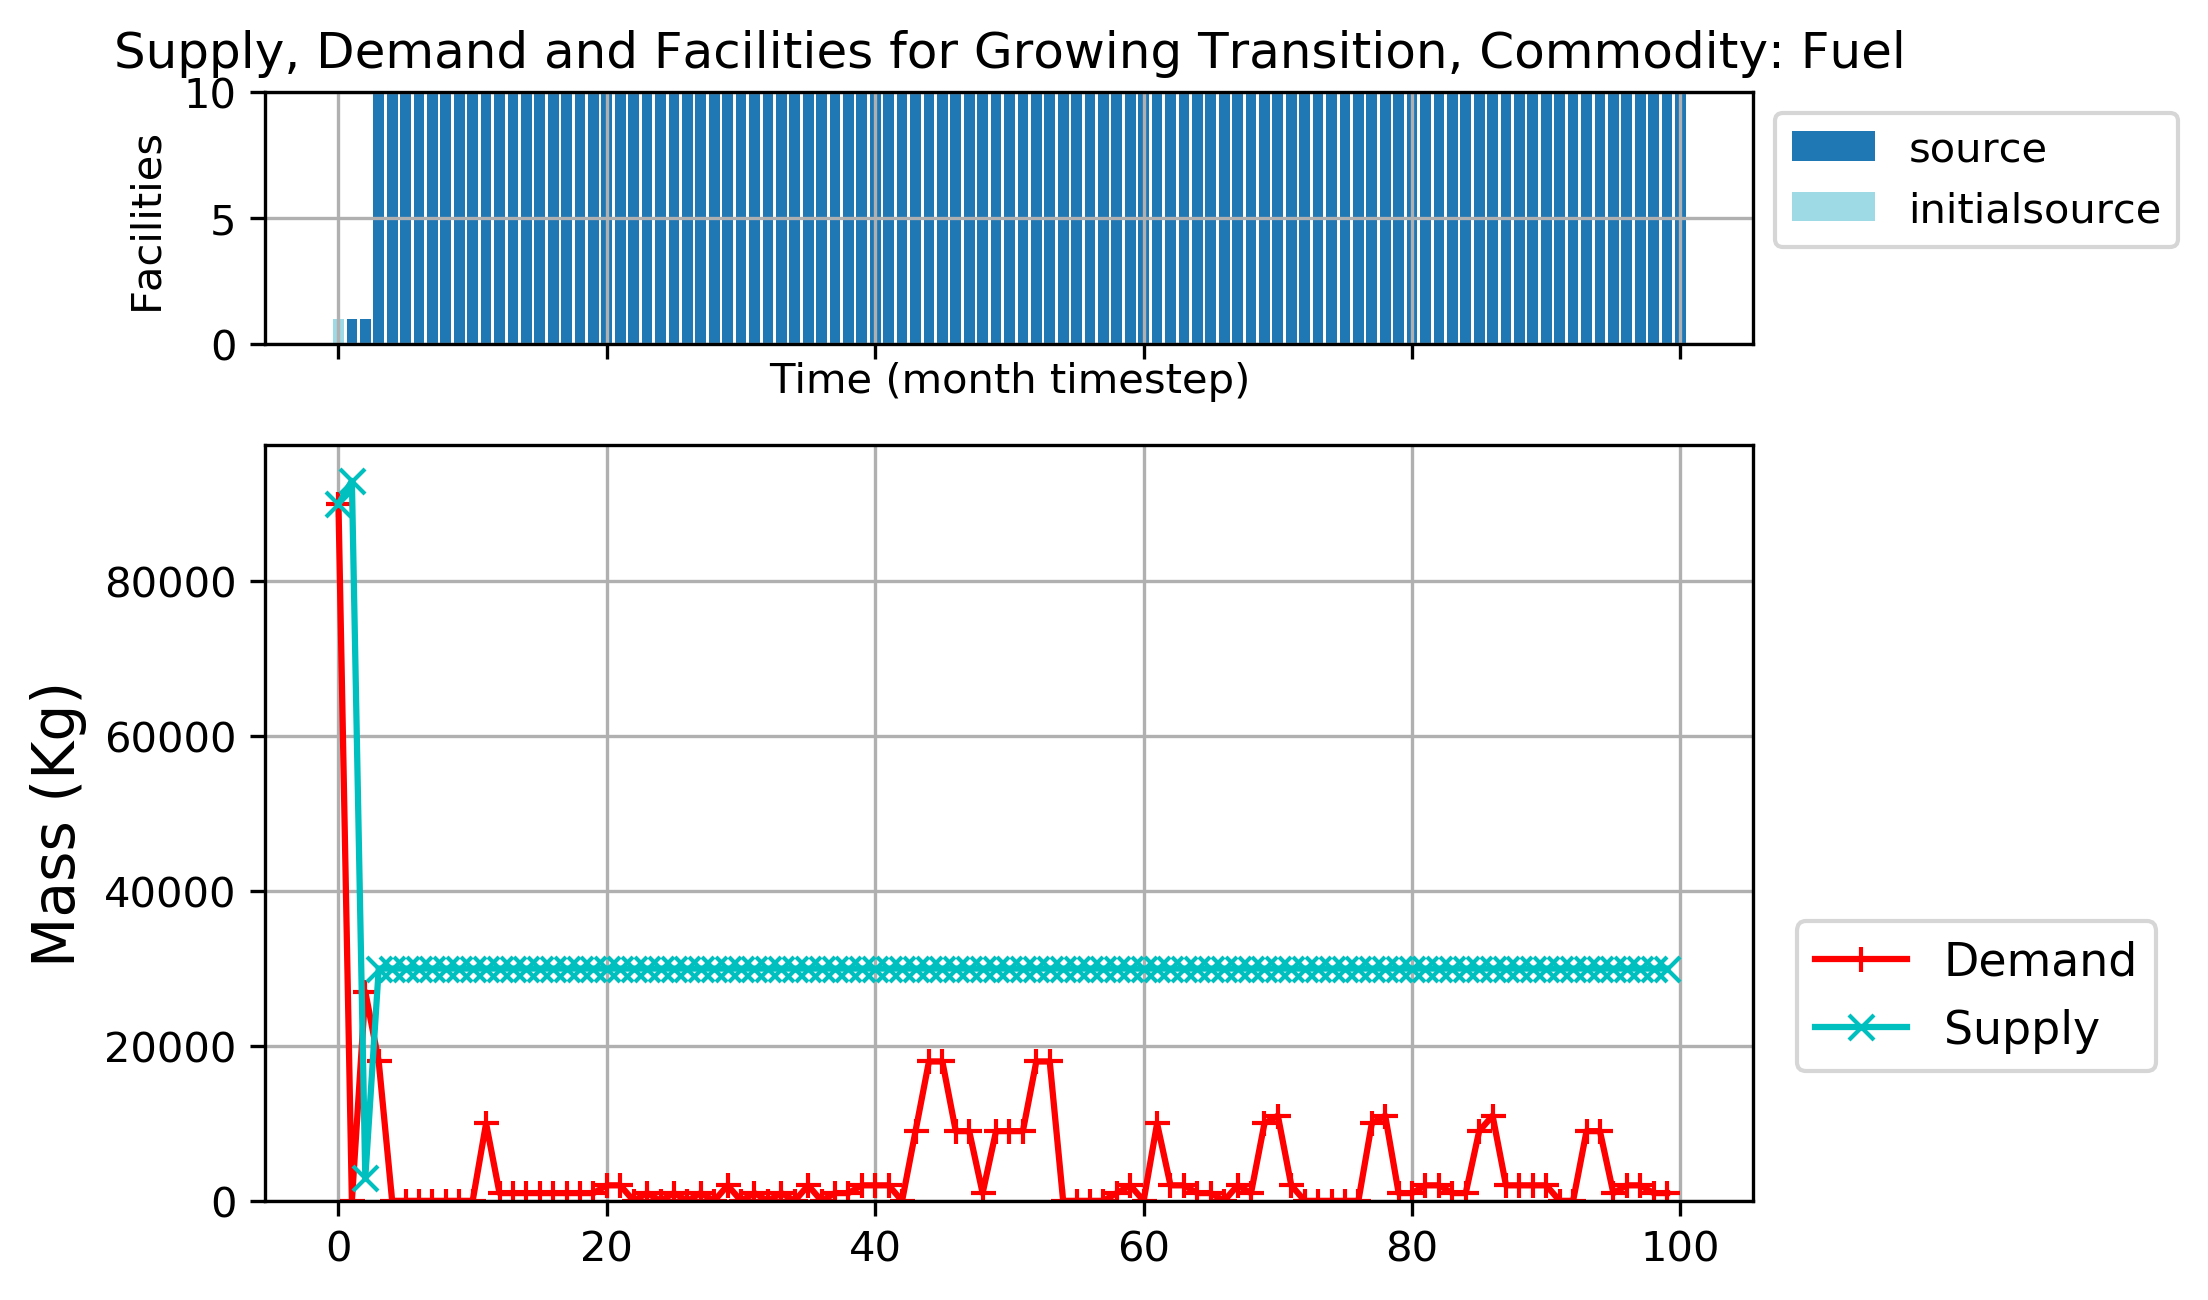
\includegraphics[width=0.9\linewidth]{figures/growingtransition-fuel.png} 
            \caption{Fuel demand and supply, and source facility deployment plot.
            Fuel is demanded by reactors and supplied by source facilities.
            There is only one time step with undersupply of fuel.}
            \label{fig:growingtransition-fuel}
        \end{subfigure}
        \begin{subfigure}[t]{\textwidth}
            \centering
            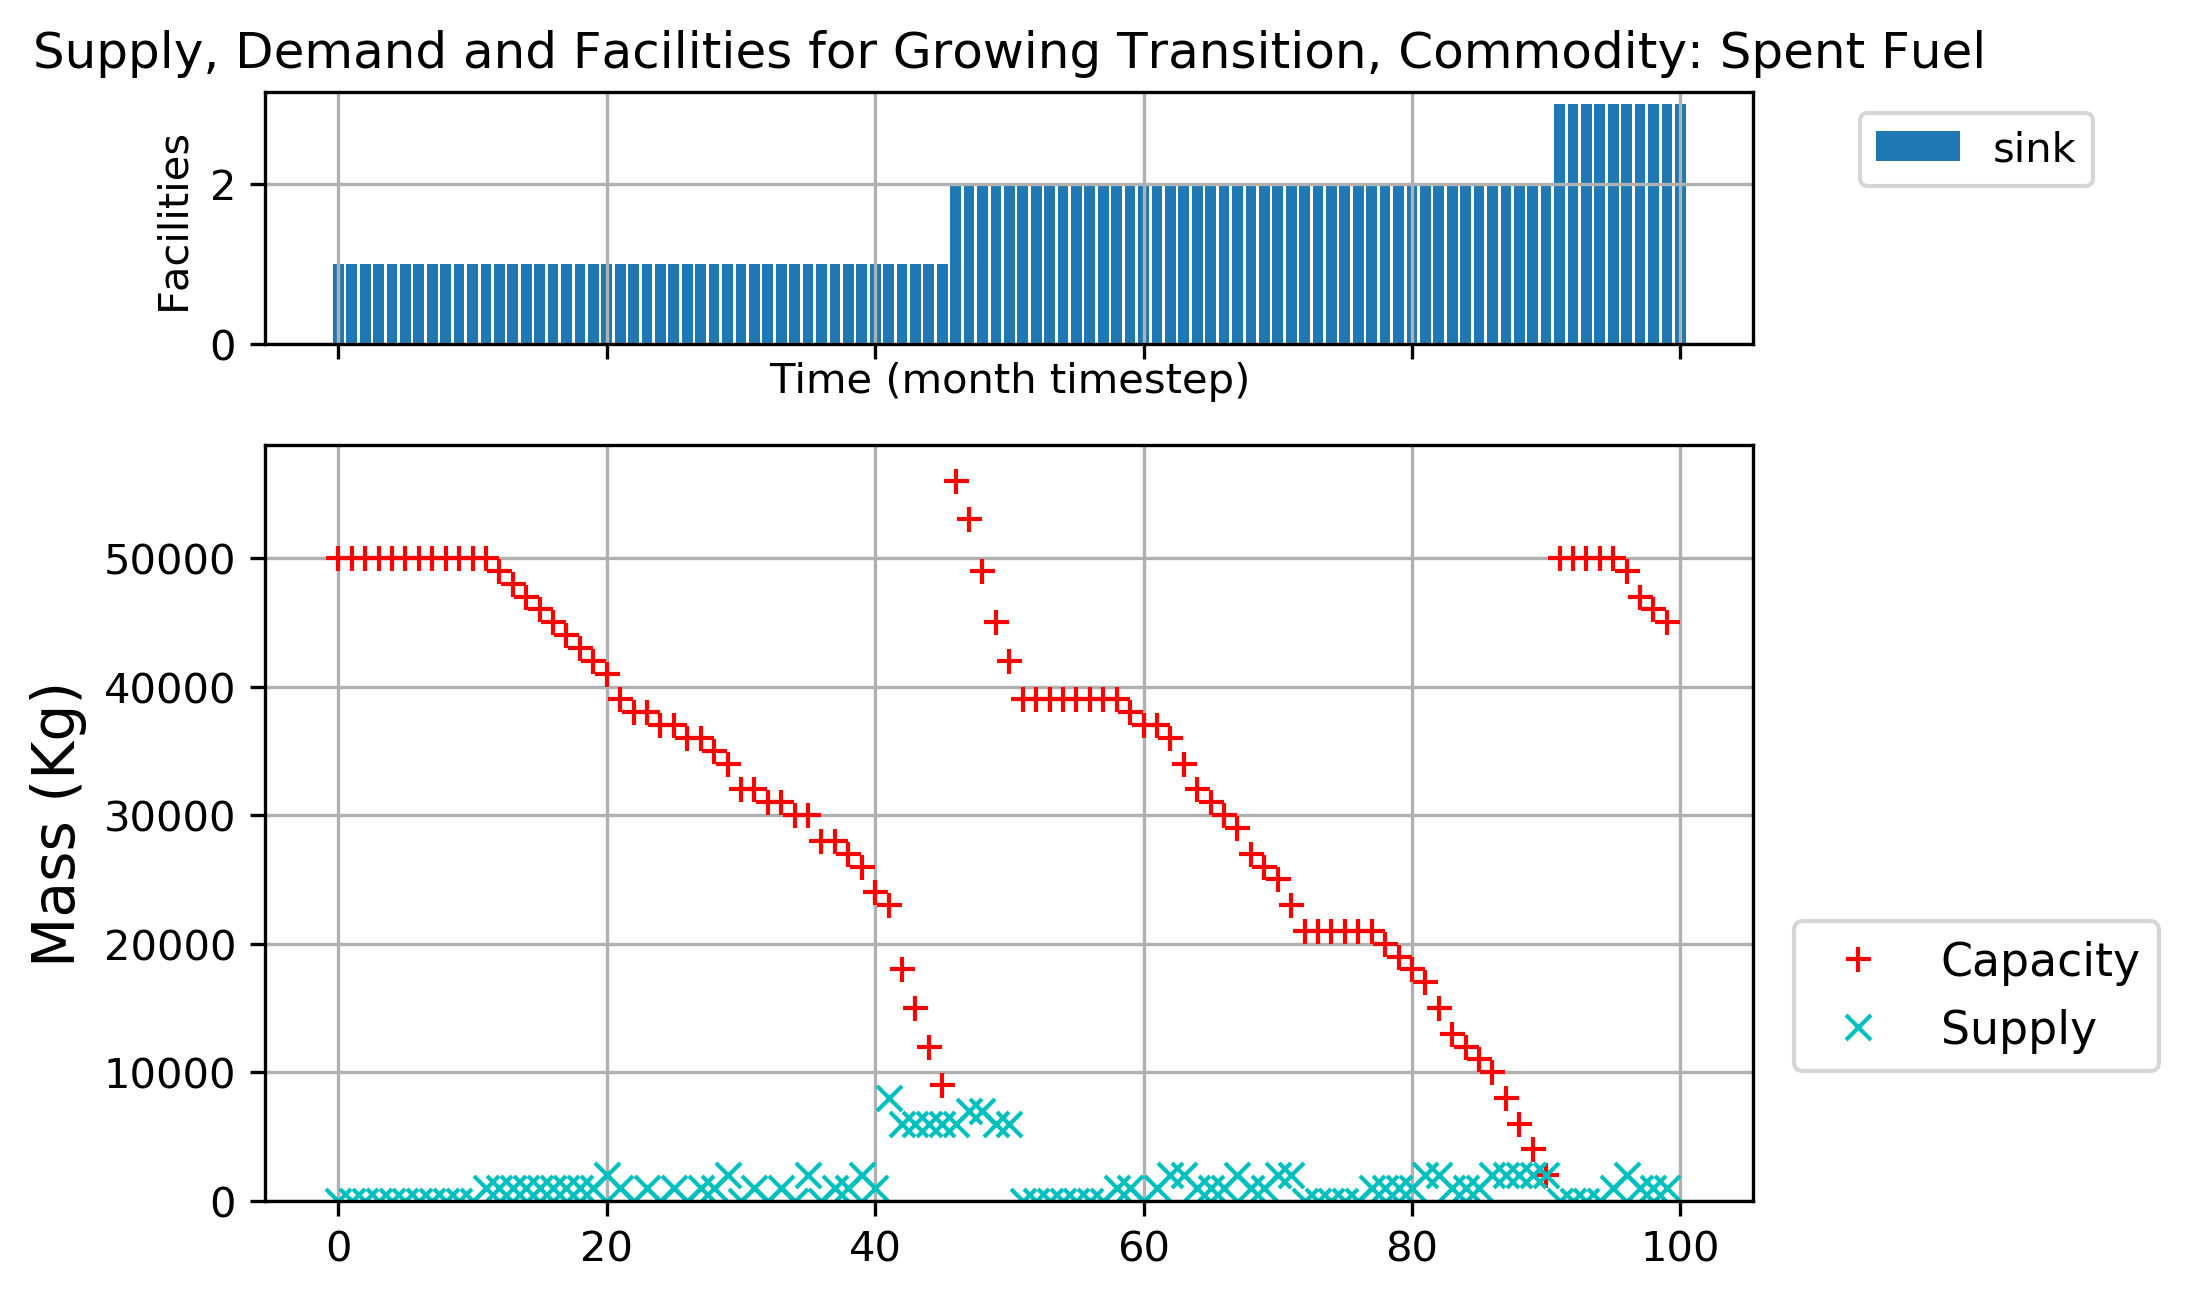
\includegraphics[width=0.9\linewidth]{figures/growingtransition-spentfuel.png} 
            \caption{Spent fuel demand and supply, and sink facility deployment plot.
                Spent Fuel is supplied by reactors and the capacity to store them 
                is provided by sink facilities.
            There are no time steps with under-capacity of sink space.}
            \label{fig:growingtransition-spentfuel}
        \end{subfigure}
        \caption{Simple linearly increasing power demand transition scenario with 
        three facility types: \texttt{source}, \texttt{reactor}, and \texttt{sink}.}
    \end{figure}
    
    \subsection{Simple Transition Scenario Simulation: Sinusoidal Demand}
    Sinusoidal power demand is the reflection of power demand in 
    the real world in which power usage is higher in the winter and summer
    and lower in the spring and fall. 
    Figures \ref{fig:sinetransition-power}, \ref{fig:sinetransition-fuel},
    and \ref{fig:sinetransition-spentfuel} demonstrate \deploy's capability 
    to deploy reactor and supporting facilities to minimize undersupply 
    when meeting linearly increasing power demand and subsequent secondary 
    commodities demand. 
    Table \ref{tab:transition-scenario-results} shows the number of 
    undersupplied timesteps.
    For a sinusoidal power demand, using the 
    \texttt{holt-winters} method to predict demand minimizes 
    power undersupply more effectively than the \texttt{FFT} method. 
    This is because the \texttt{holt-winters} method excels in
    forecasting data points for repetitive seasonal series of data. 

    \begin{figure}[]
        \centering
        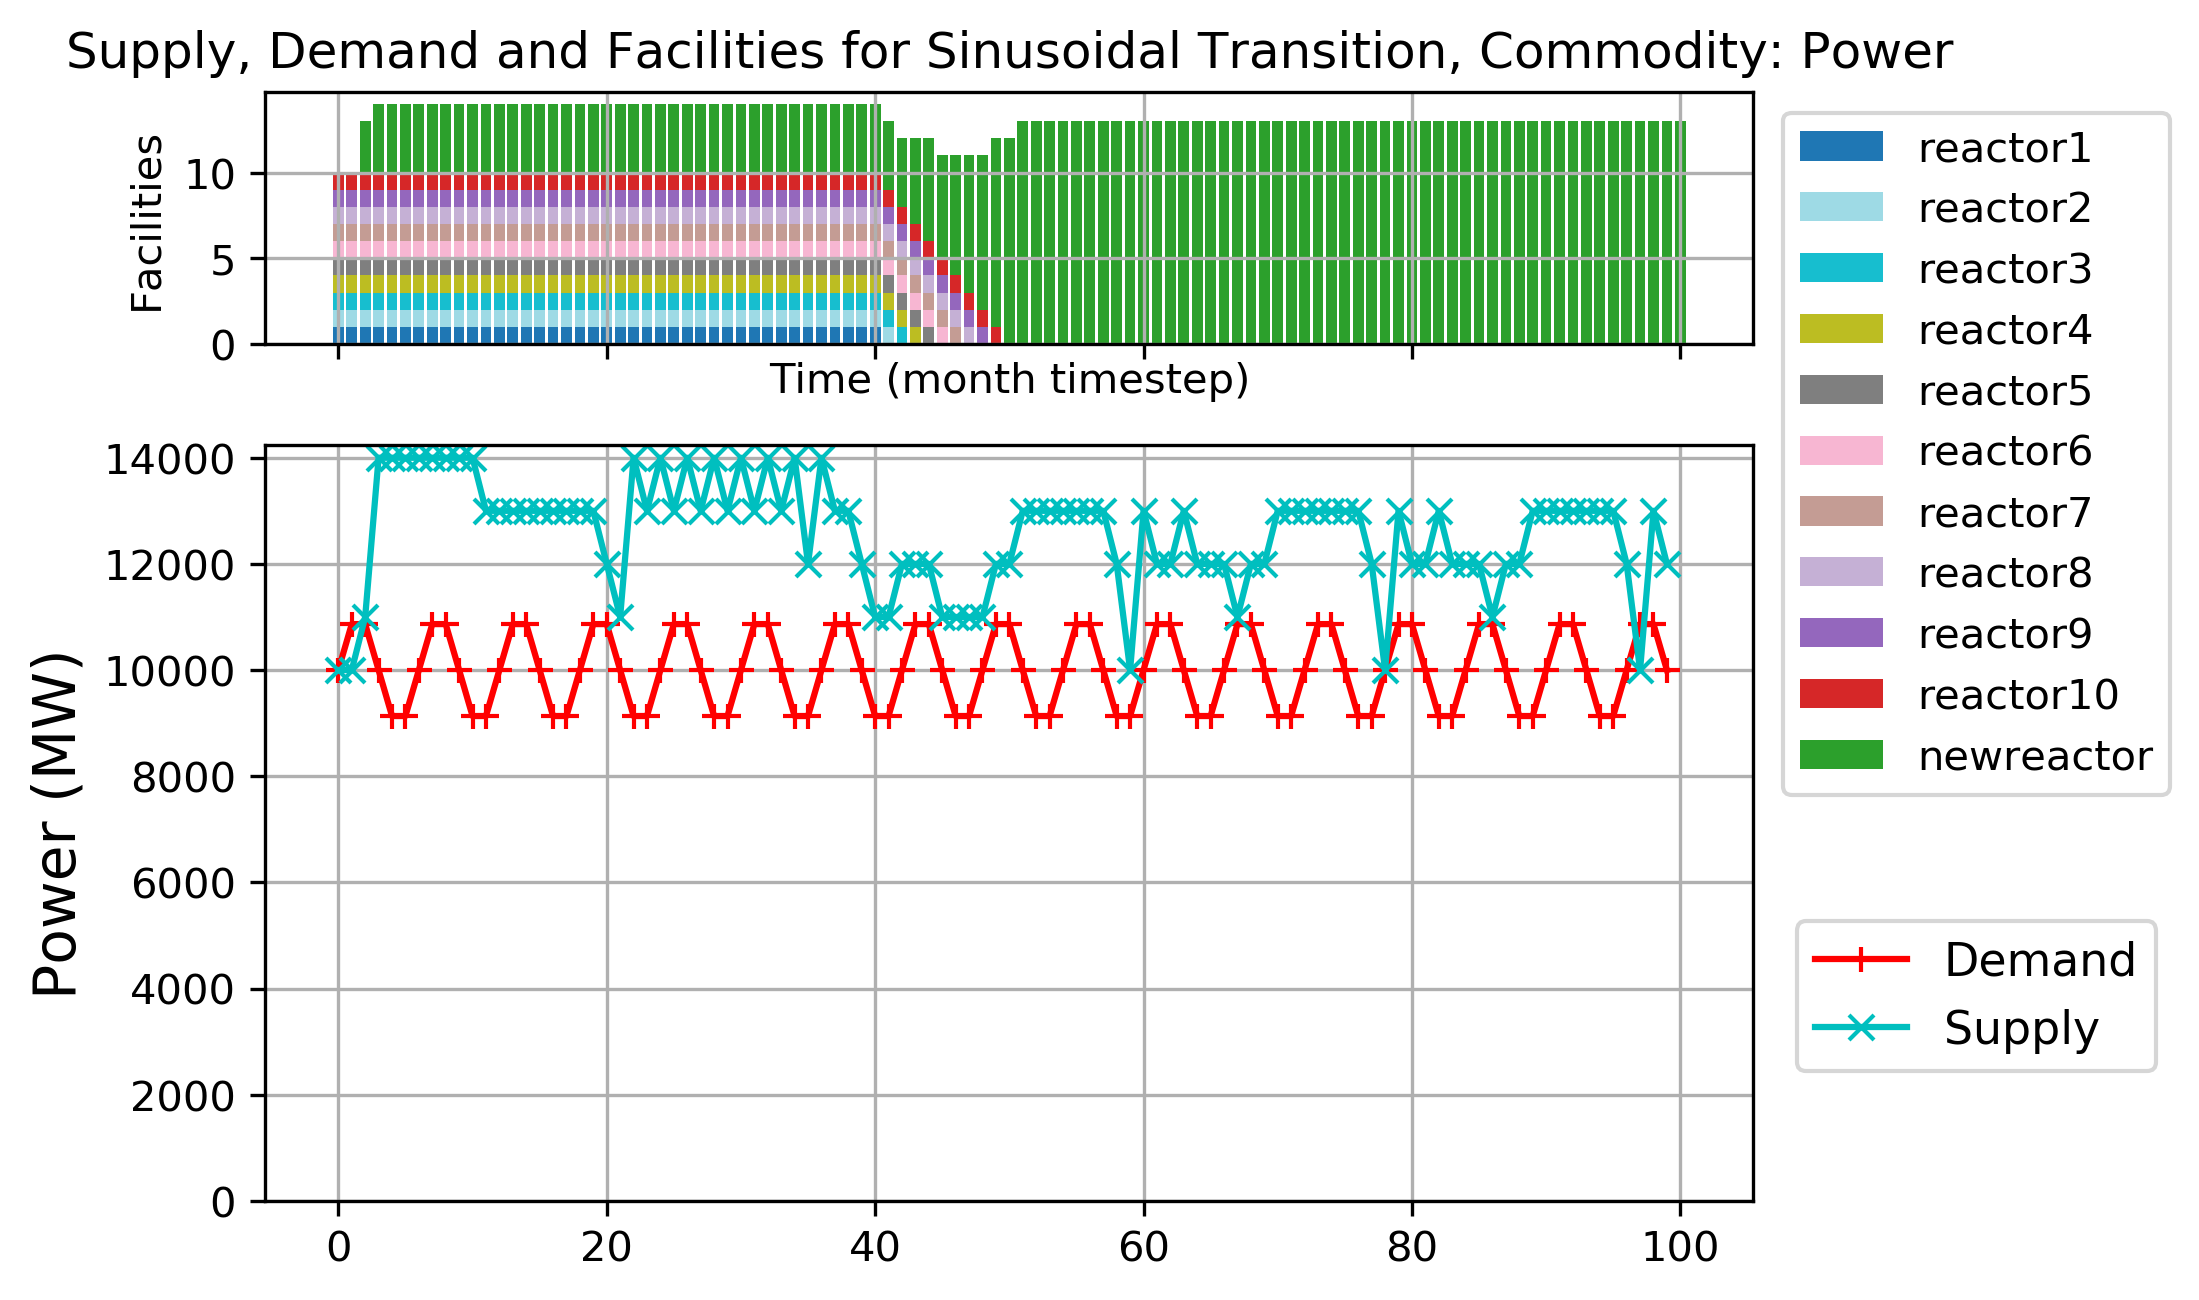
\includegraphics[width=0.9\linewidth]{figures/sinetransition-power.png} 
            \caption{Power demand and supply, and reactor facility deployment plot for  
            a simple sinusoidal power demand transition scenario with 
            three facility types: \texttt{source}, \texttt{reactor}, and \texttt{sink}.
            Power demand is a user-defined equation and power is supplied by the reactors.
            There are no time steps with undersupply of power.}
            \label{fig:sinetransition-power}
    \end{figure}
    
    \begin{figure}[]
        \centering
        \begin{subfigure}[t]{\textwidth}
            \centering
            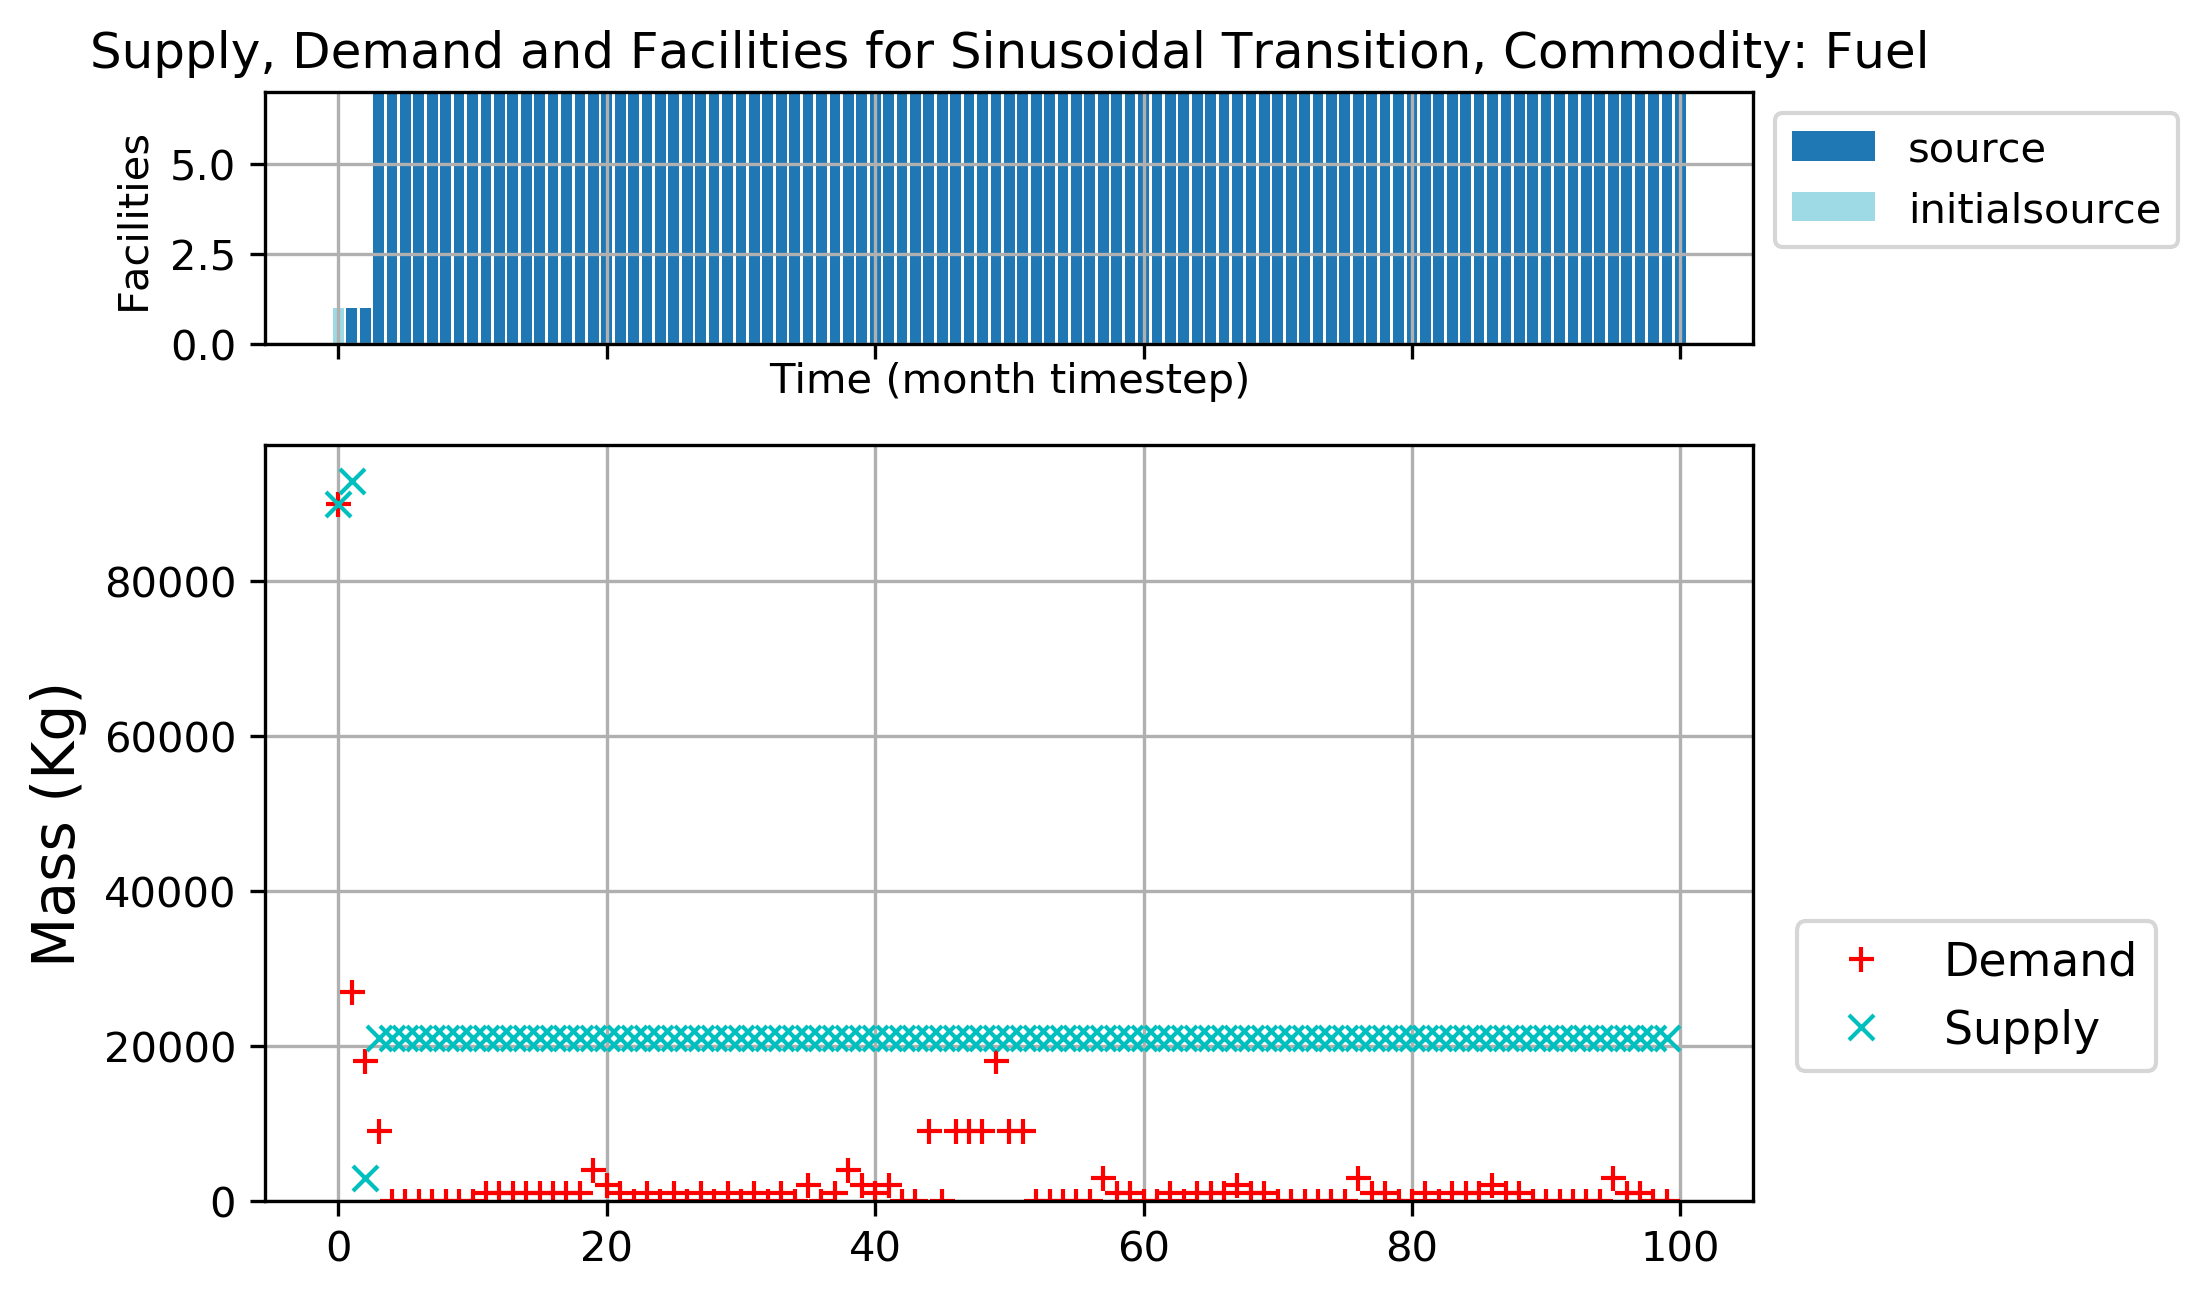
\includegraphics[width=0.9\linewidth]{figures/sinetransition-fuel.png} 
            \caption{Fuel demand and supply, and source facility deployment plot.
            Fuel is demanded by reactors and supplied by source facilities.
            There is only one time step with undersupply of fuel.}
            \label{fig:sinetransition-fuel}
        \end{subfigure}
        \begin{subfigure}[t]{\textwidth}
            \centering
            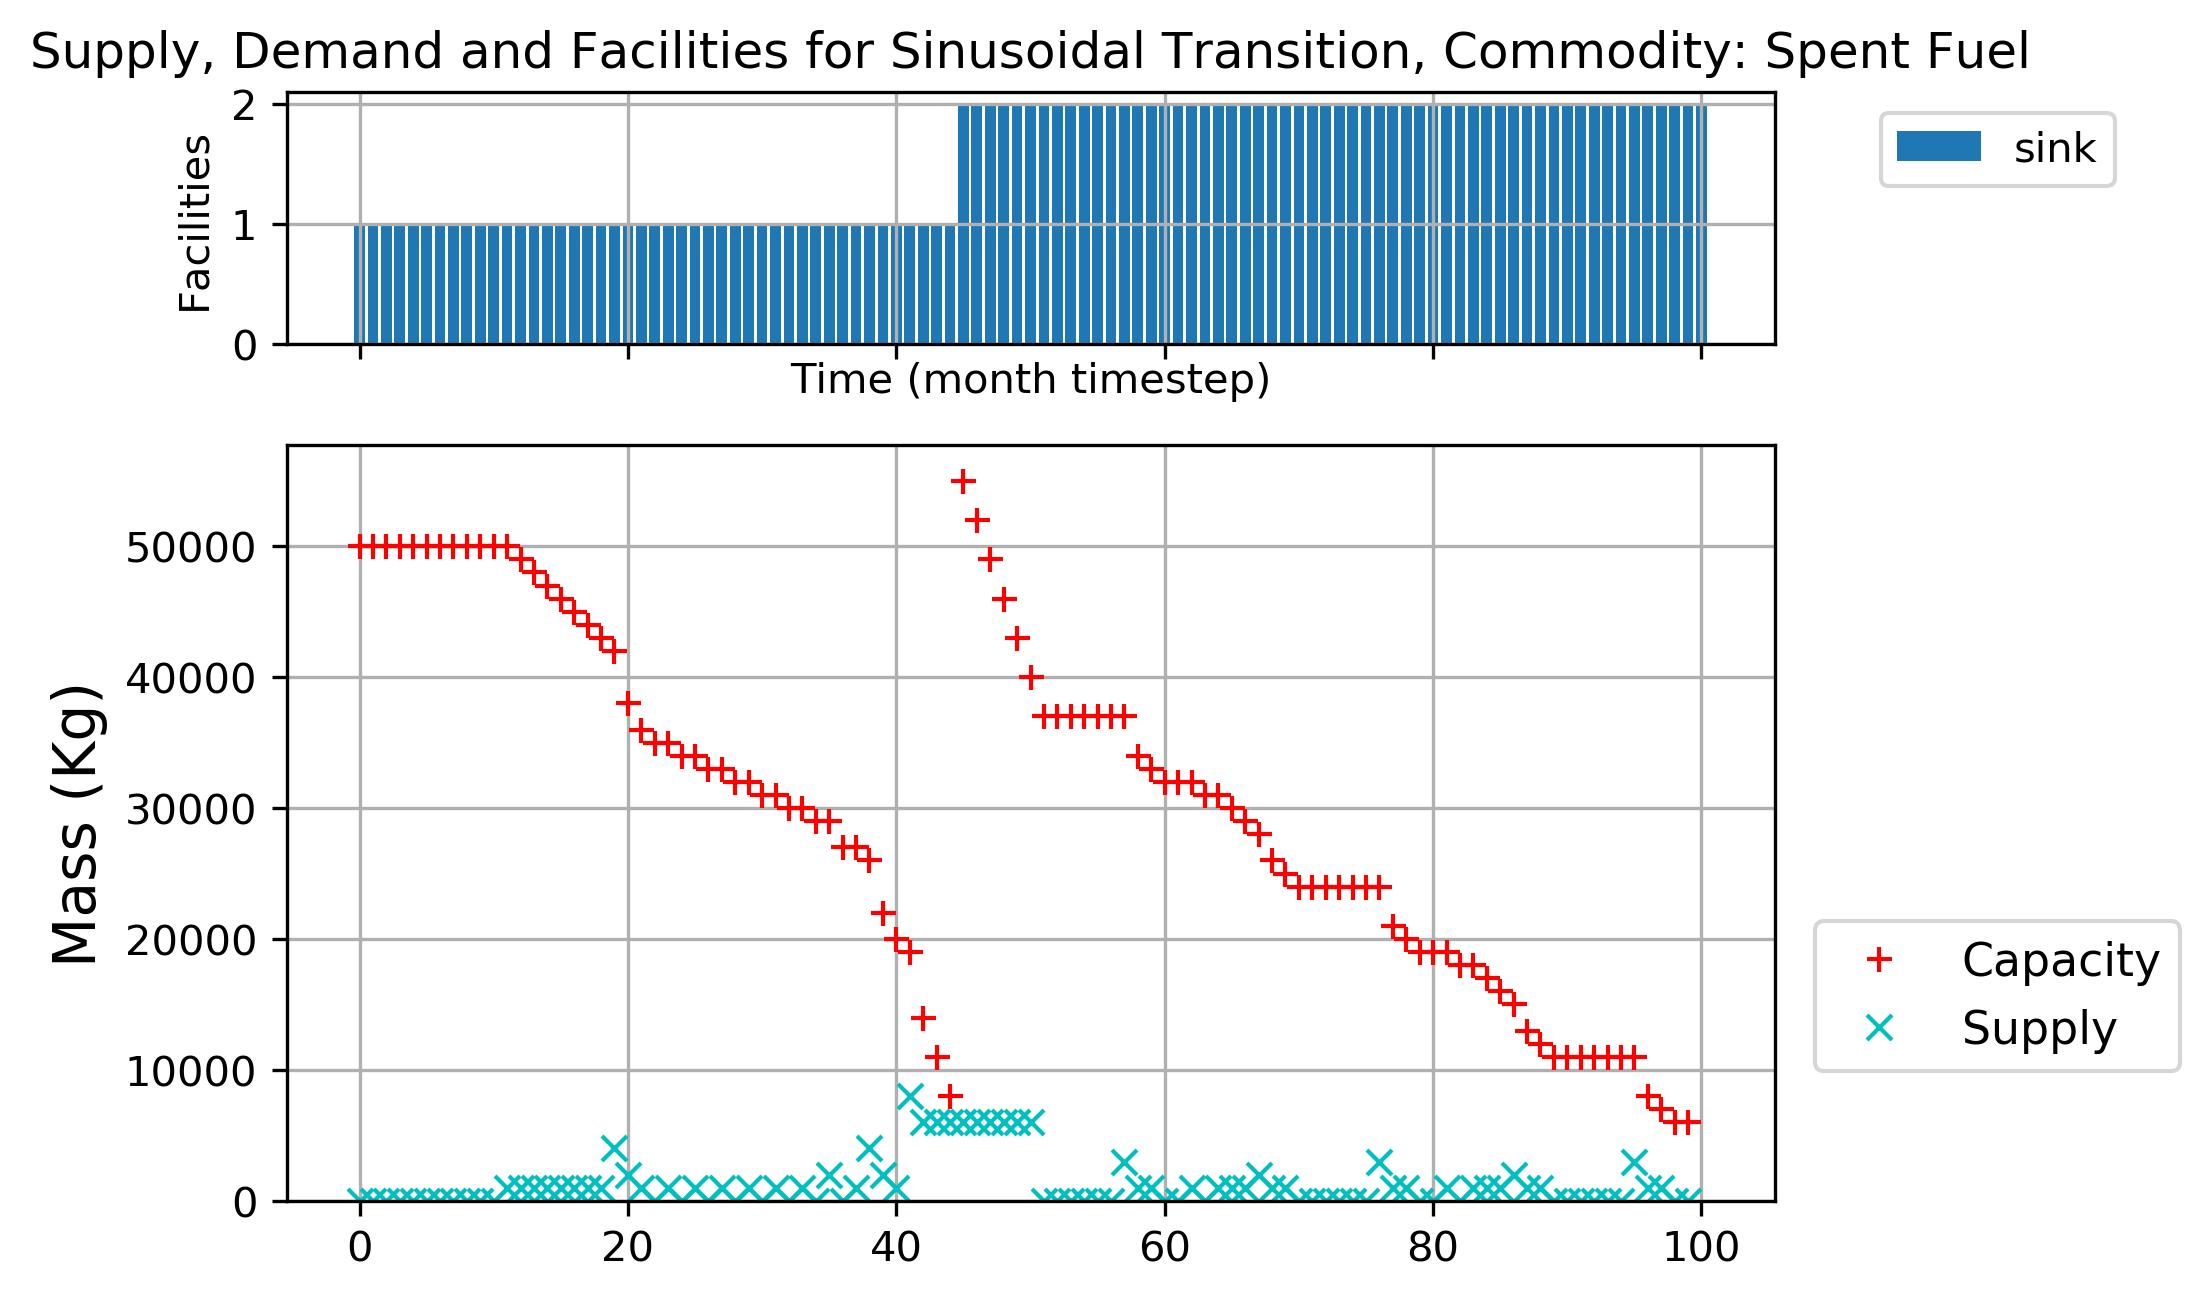
\includegraphics[width=0.9\linewidth]{figures/sinetransition-spentfuel.png} 
            \caption{Spent fuel demand and supply, and sink facility deployment plot.
                Spent Fuel is supplied by reactors and the capacity to store them 
                is provided by sink facilities.
            There are no time steps with under-capacity of sink space.}
            \label{fig:sinetransition-spentfuel}
        \end{subfigure}
        \caption{Simple sinusoidal power demand transition scenario with 
        three facility types: \texttt{source}, \texttt{reactor}, and \texttt{sink}.}
    \end{figure}

    \begin{table}[]
        \centering
        \doublespacing
        \caption {The total number of time steps with commodity undersupply 
        for each simple transition scenario. }
        \label{tab:transition-scenario-results}
            \small
            \begin{tabular}{l|rr}	
                \hline
                \textbf{Simple Transition Scenario}    & \textbf{Commodity}    & \textbf{No. of time steps} \\ 
                && \textbf{with undersupply} \\ \hline
                \multirow{3}{*}{\textbf{Constant Power}} & Fuel & 1 \\ 
                                                         & Power & 0 \\ 
                                                         & Spent Fuel & 0 \\ \hline
                \multirow{3}{*}{\textbf{Linearly Increasing Power}} & Fuel & 1 \\ 
                                                         & Power & 0 \\ 
                                                         & Spent Fuel & 0 \\ \hline
                \multirow{3}{*}{\textbf{Sinusoidal Power}} & Fuel & 1 \\ 
                                                         & Power & 1 \\ 
                                                         & Spent Fuel & 0 \\ \hline
                \end{tabular}
    \end{table}

\section{\deploy Demonstration of EG01-30 Transition Scenario} 
\label{sec:eg01-30}
Figure \ref{fig:30flow} shows the setup of facilities and mass flows 
for EG01-30 in \Cyclus. 
In the EG01-30 transition scenario, the initial LWR fleet 
progressively decommissions at the 80-year mark,
after which \deploy deploys \glspl{SFR} and \gls{MOX} \glspl{LWR} to 
meet a linearly increasing power demand. 
Transuranic elements from the spent fuel are recycled to 
produce \gls{MOX} \gls{LWR} and \gls{SFR} fuel. 
The power demand equation (t represents a month): 
\begin{align}
    P(t) = 60000 + \frac{250t}{12}\ MW
\end{align}

\begin{figure}[]
    \centering
    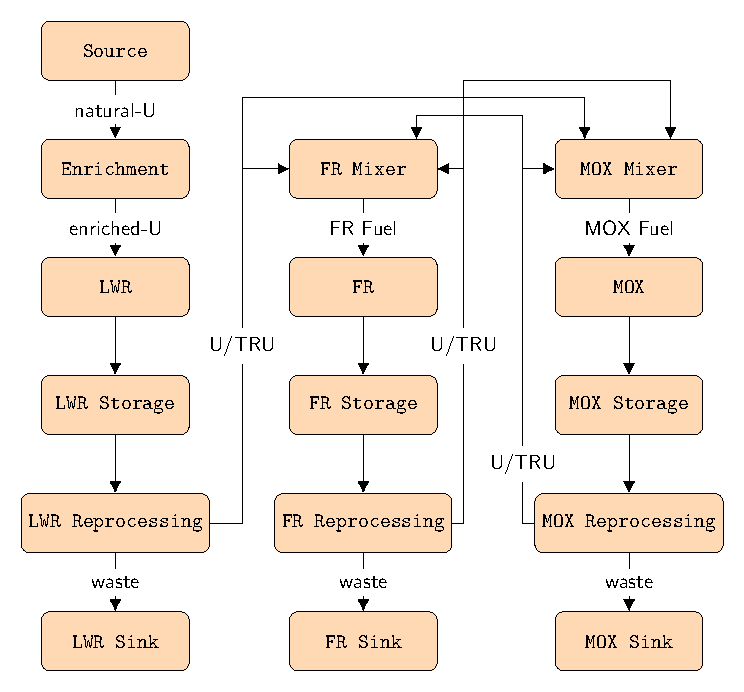
\includegraphics[width=\linewidth]{30flow.pdf} 
    \caption{Facility and mass flow for EG01-30 transition scenario.}
    \label{fig:30flow}
\end{figure}

We conducted a comparison study of different prediction 
methods and power supply buffer sizes to determine the 
optimal \deploy parameters to minimize 
power undersupply in the EG01-30 \Cyclus 
transition scenario. 
The subsequent sections discuss the results from the comparison 
study. 

\subsection{Comparison of Prediction Methods}
We ran EG01-30 transition scenarios with different prediction 
methods to determine the prediction method that best minimizes 
power undersupply. 
In Figure \ref{fig:eg30under}, each histogram represents 
the number of time steps with undersupply or 
under capacity for all commodities for each prediction method.  
Table \ref{tab:all-power} shows the number of time steps with power 
undersupply for the linearly increasing power EG01-30 transition scenario. 
Figure \ref{fig:eg30under} and Table \ref{tab:all-power}
demonstrate that the \texttt{FFT} and \texttt{POLY} methods 
perform the best for the EG01-30 transition scenario, 
with the least number of time steps with power undersupply.

\begin{figure}[]
	\centering
	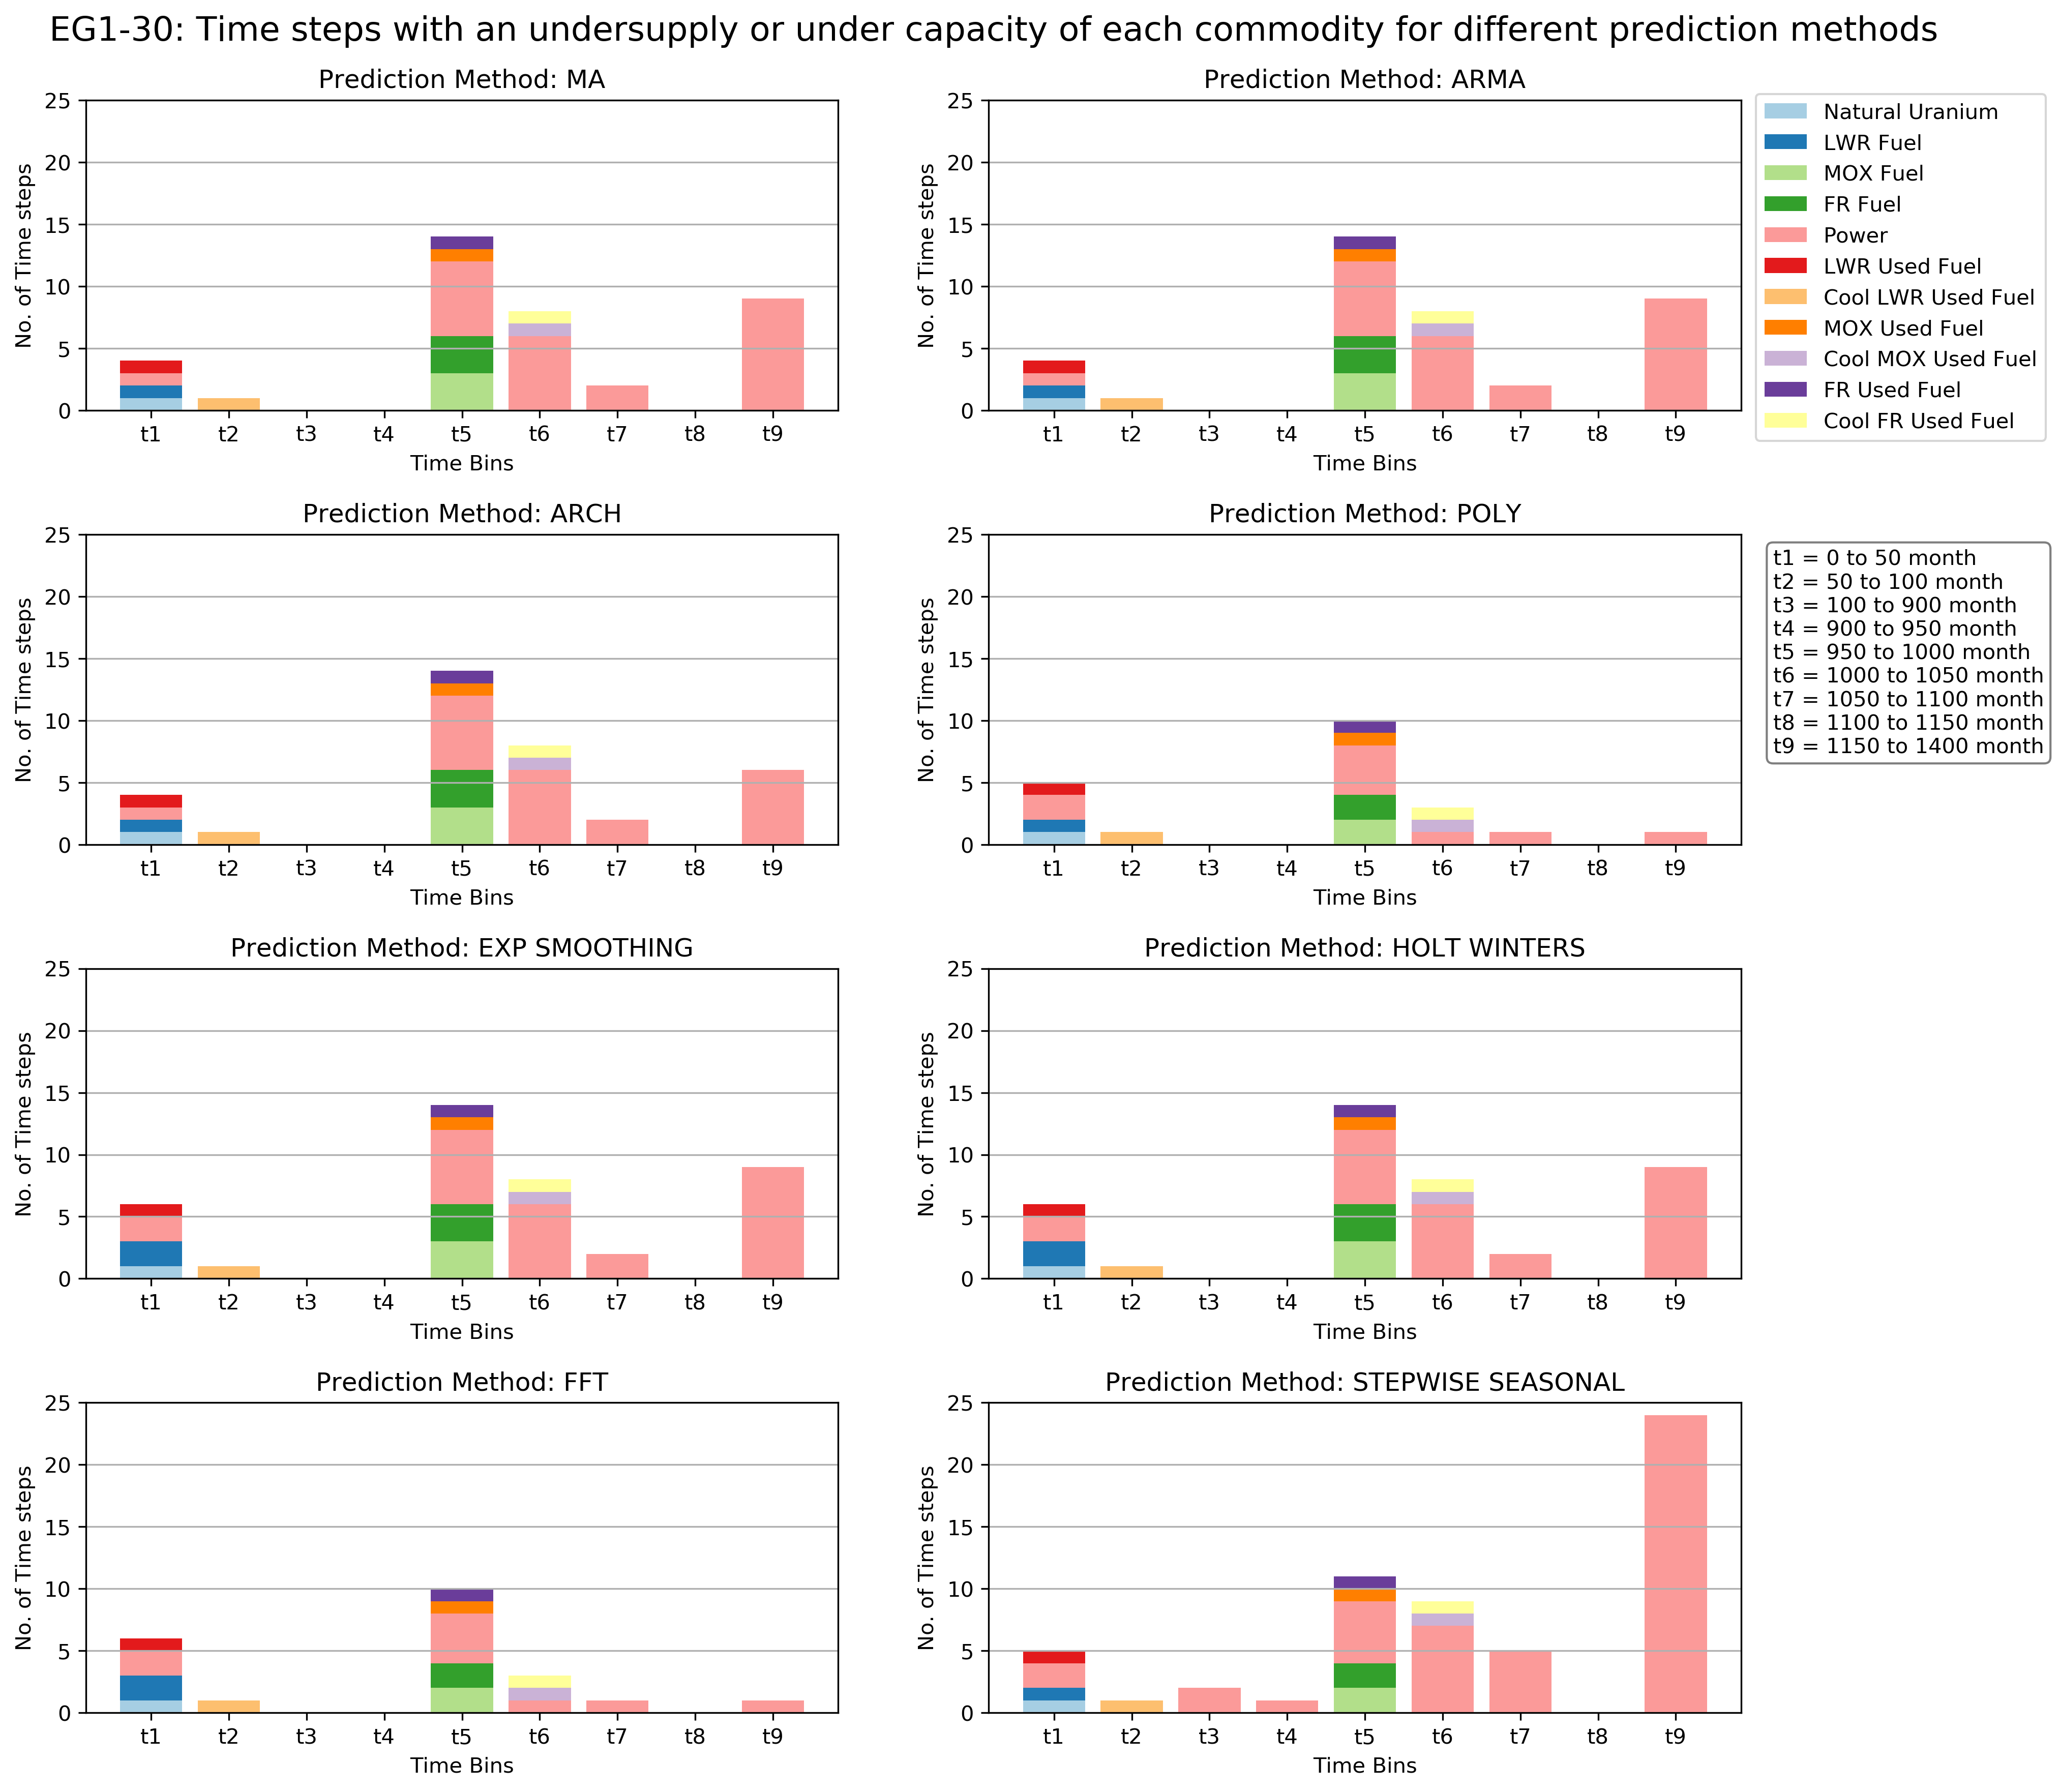
\includegraphics[width=1.1\linewidth]{eg01-30-histogram.png} 
	\caption{
	EG01-30 transition scenario with linearly increasing power demand. 
	Each subplot shows the total number of time steps in which there exists 
	undersupply and under capacity of commodities for each prediction method. 
	The different colors represent different commodities, and each time bin 
	refers to a specific time periods in the simulation.
    The \texttt{FFT} and \texttt{POLY} prediction methods perform the best, 
    with the least number of 
	time steps with undersupply and under capacity.}
	\label{fig:eg30under}
\end{figure}

\begin{table}[]
    \doublespacing
	\centering
        \caption{Total number of time steps with undersupply of power for the 
        EG01-30 transition scenario for different prediction methods.}
		\label{tab:all-power}
		\small
        \begin{tabular}{lr}
		\hline
        \textbf{Algorithm} & \textbf{EG01-30: No. of Time Steps} \\ 
        & \textbf{with Power Undersupply} \\ \hline
		\texttt{MA}     		& 24 \\ 
		\texttt{ARMA}     	    & 24\\ 
		\texttt{ARCH}     	    & 21\\ 
		\texttt{POLY}      		&  9\\ 
		\texttt{EXP-SMOOTHING} 	& 25\\ 
		\texttt{HOLT-WINTERS}  	& 25\\ 
		\texttt{FFT}       		& 9\\ 
		\texttt{SW-SEASONAL}    & 51\\ \hline
	\end{tabular}
\end{table}


\subsection{Comparison of Power Buffer Sizes}
For the EG01-30 linearly increasing power demand 
transition scenario, the power buffer size is varied
for both \texttt{FFT} and \texttt{POLY} methods. 
Varying the power buffer size does not impact the number of 
undersupply time steps for the transition scenario 
with the \texttt{POLY} prediction method.
Whereas, for the transition scenario with \texttt{FFT} prediction method, 
Figure \ref{fig:eg30-bufplot} and Table \ref{tab:buff_size} 
show that with increased buffer size, the number of 
power undersupply time steps decreases. 
The cumulative undersupply is the smallest for a buffer 
size of 8000MW.  
These undersupply time 
steps occur at the beginning of the simulation and for one 
time step when the transition begins. 
This is expected since without time series data 
at the beginning of the simulation, \deploy takes a few 
time steps to collect time series data about power demand 
to predict and start deploying reactor and supporting 
fuel cycle facilities. 
Therefore, a buffer of 8000MW minimizes 
the power undersupply for the EG01-EG30 transition scenario
with the \texttt{FFT} prediction method.

\begin{figure}[]
		\centering
		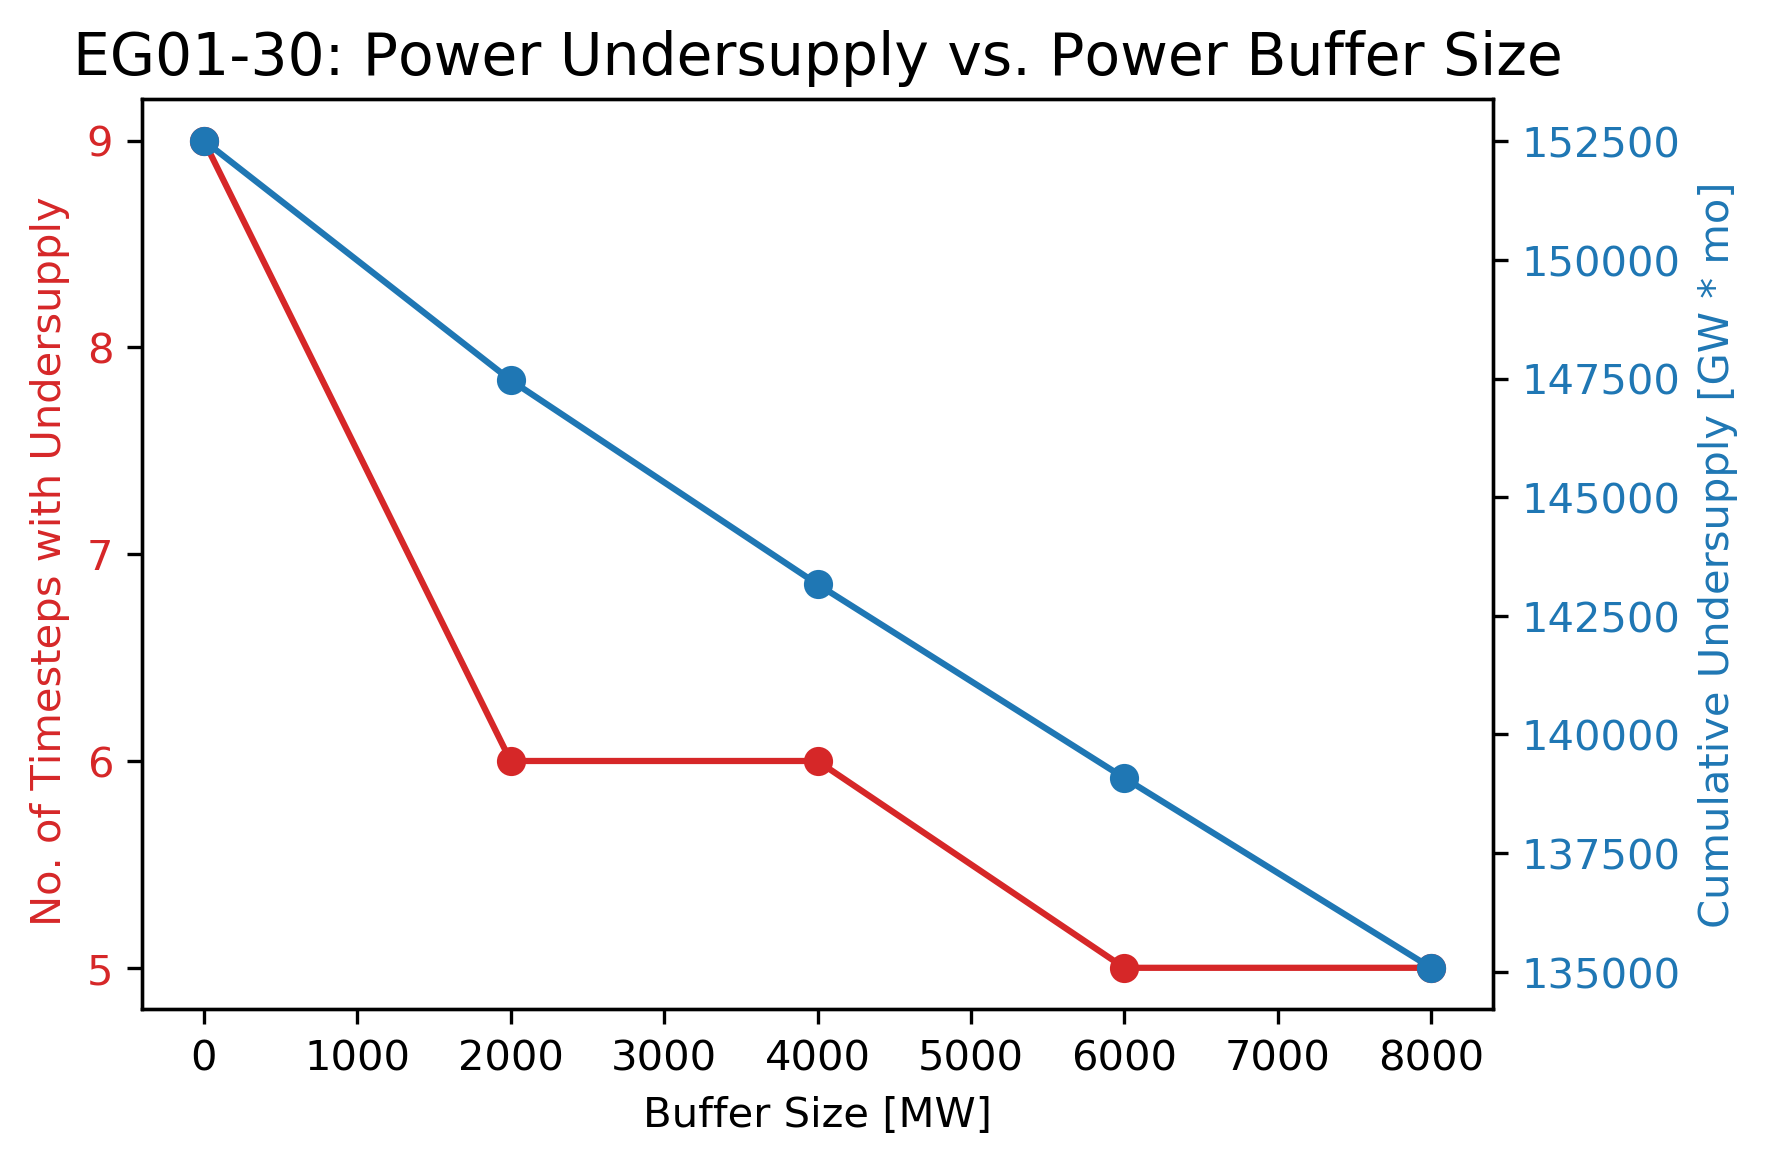
\includegraphics[width=\linewidth]{30-sens-buffer.png} 
    \caption{The effect of sensitivity analysis of power buffer size on cumulative 
    undersupply of power for the EG01-30 transition scenario with linearly 
    increasing power demand using the \texttt{FFT} method.}
    \label{fig:eg30-bufplot}
\end{figure}

\begin{table}[h]
    \centering
    \doublespacing
	\caption{Dependency of the power undersupply on the buffer size 
	for EG01-EG30 transition scenarios with linearly 
    increasing power demand using the \texttt{FFT} prediction method.
    There is less power undersupply for a larger power buffer size.}
	\label{tab:buff_size}
	\small
	\begin{tabular}{rrr}
                \hline
                \textbf{Buffer [MW]}     & \textbf{Undersupply}               & \textbf{EG01-30} \\
		\hline
		\textbf{0}             & Time steps $[\#]$  & 9\\  
                      & Cumulative $[GW\cdot mo]$    & 152517 \\ \hline
        \textbf{2000}          & Undersupplied $[\#]$ & 6 \\  
        	      & Cumulative $[GW\cdot mo]$   & 147166 \\ \hline
        \textbf{4000}         & Time steps $[\#]$ & 6 \\  
				  & Cumulative $[GW\cdot mo]$     & 143166 \\ \hline
        \textbf{6000}          & Time steps $[\#]$  & 5 \\  
		& Cumulative $[GW\cdot mo]$     & 139083 \\ \hline
        \textbf{8000}          & Time steps $[\#]$  & 5  \\  
	              & Cumulative $[GW\cdot mo]$  & 135083 \\ \hline
	\end{tabular}
\end{table}

\subsection{Demonstration of Best Performance Model}
Table \ref{tab:bestinputs} 
shows \deploy input parameters for the 
EG01-EG30 transition scenario
that minimizes undersupply of power and minimizes 
the undersupply and under capacity of the other commodities
in the simulation. 
The need for commodity buffers is a reflection of reality
in which a supply buffer is usually maintained to ensure 
continuity in the event of an unexpected failure in the supply chain.

Figure \ref{fig:30stack} shows the
time-dependent deployment of reactor and supporting facilities 
for the EG01-30 linearly increasing power demand 
transition scenario.
\deploy automatically deploys reactor and supporting facilities 
to set up a supply chain to meet power demand
during a transition from \glspl{LWR} to \gls{MOX} \glspl{LWR} and 
\glspl{SFR} for EG01-30. 

\begin{table}[]
    \centering
    \doublespacing
    \caption{\deploy's input parameters for
	EG01-EG30 transition scenario
	that minimizes undersupply for power and minimizes 
	the undersupply and under capacity for other facilities. }
	\label{tab:bestinputs}
    \small
    \begin{tabular}{llr}
    \hline
                              & \textbf{\deploy Input Parameter}            & \textbf{EG01-30}            \\ \hline
    \multirow{4}{*}{\textbf{Required}} & Demand driving commodity   & Power              \\
                              & Demand equation {[}MW{]}   & 60000+250t/12        \\
                              & Prediction method          & \texttt{FFT}                \\
                              & Deployment driving method  & Installed Capacity \\ \cline{1-3}
    \multirow{2}{*}{\textbf{Optional}} & Buffer type                & Absolute           \\
                              & Power buffer size {[}MW{]} & 8000               \\ 
                              & Transition start date [Month] & 960 (Year 80)\\ 
                              & Fleet share percentage [\%] & \gls{MOX} \gls{PWR}: 15\%, \gls{SFR}: 85\%\\ \hline
    \end{tabular}%
    \end{table}

    \begin{figure}[]
        \centering
        \begin{subfigure}[t]{\textwidth}
            \centering
            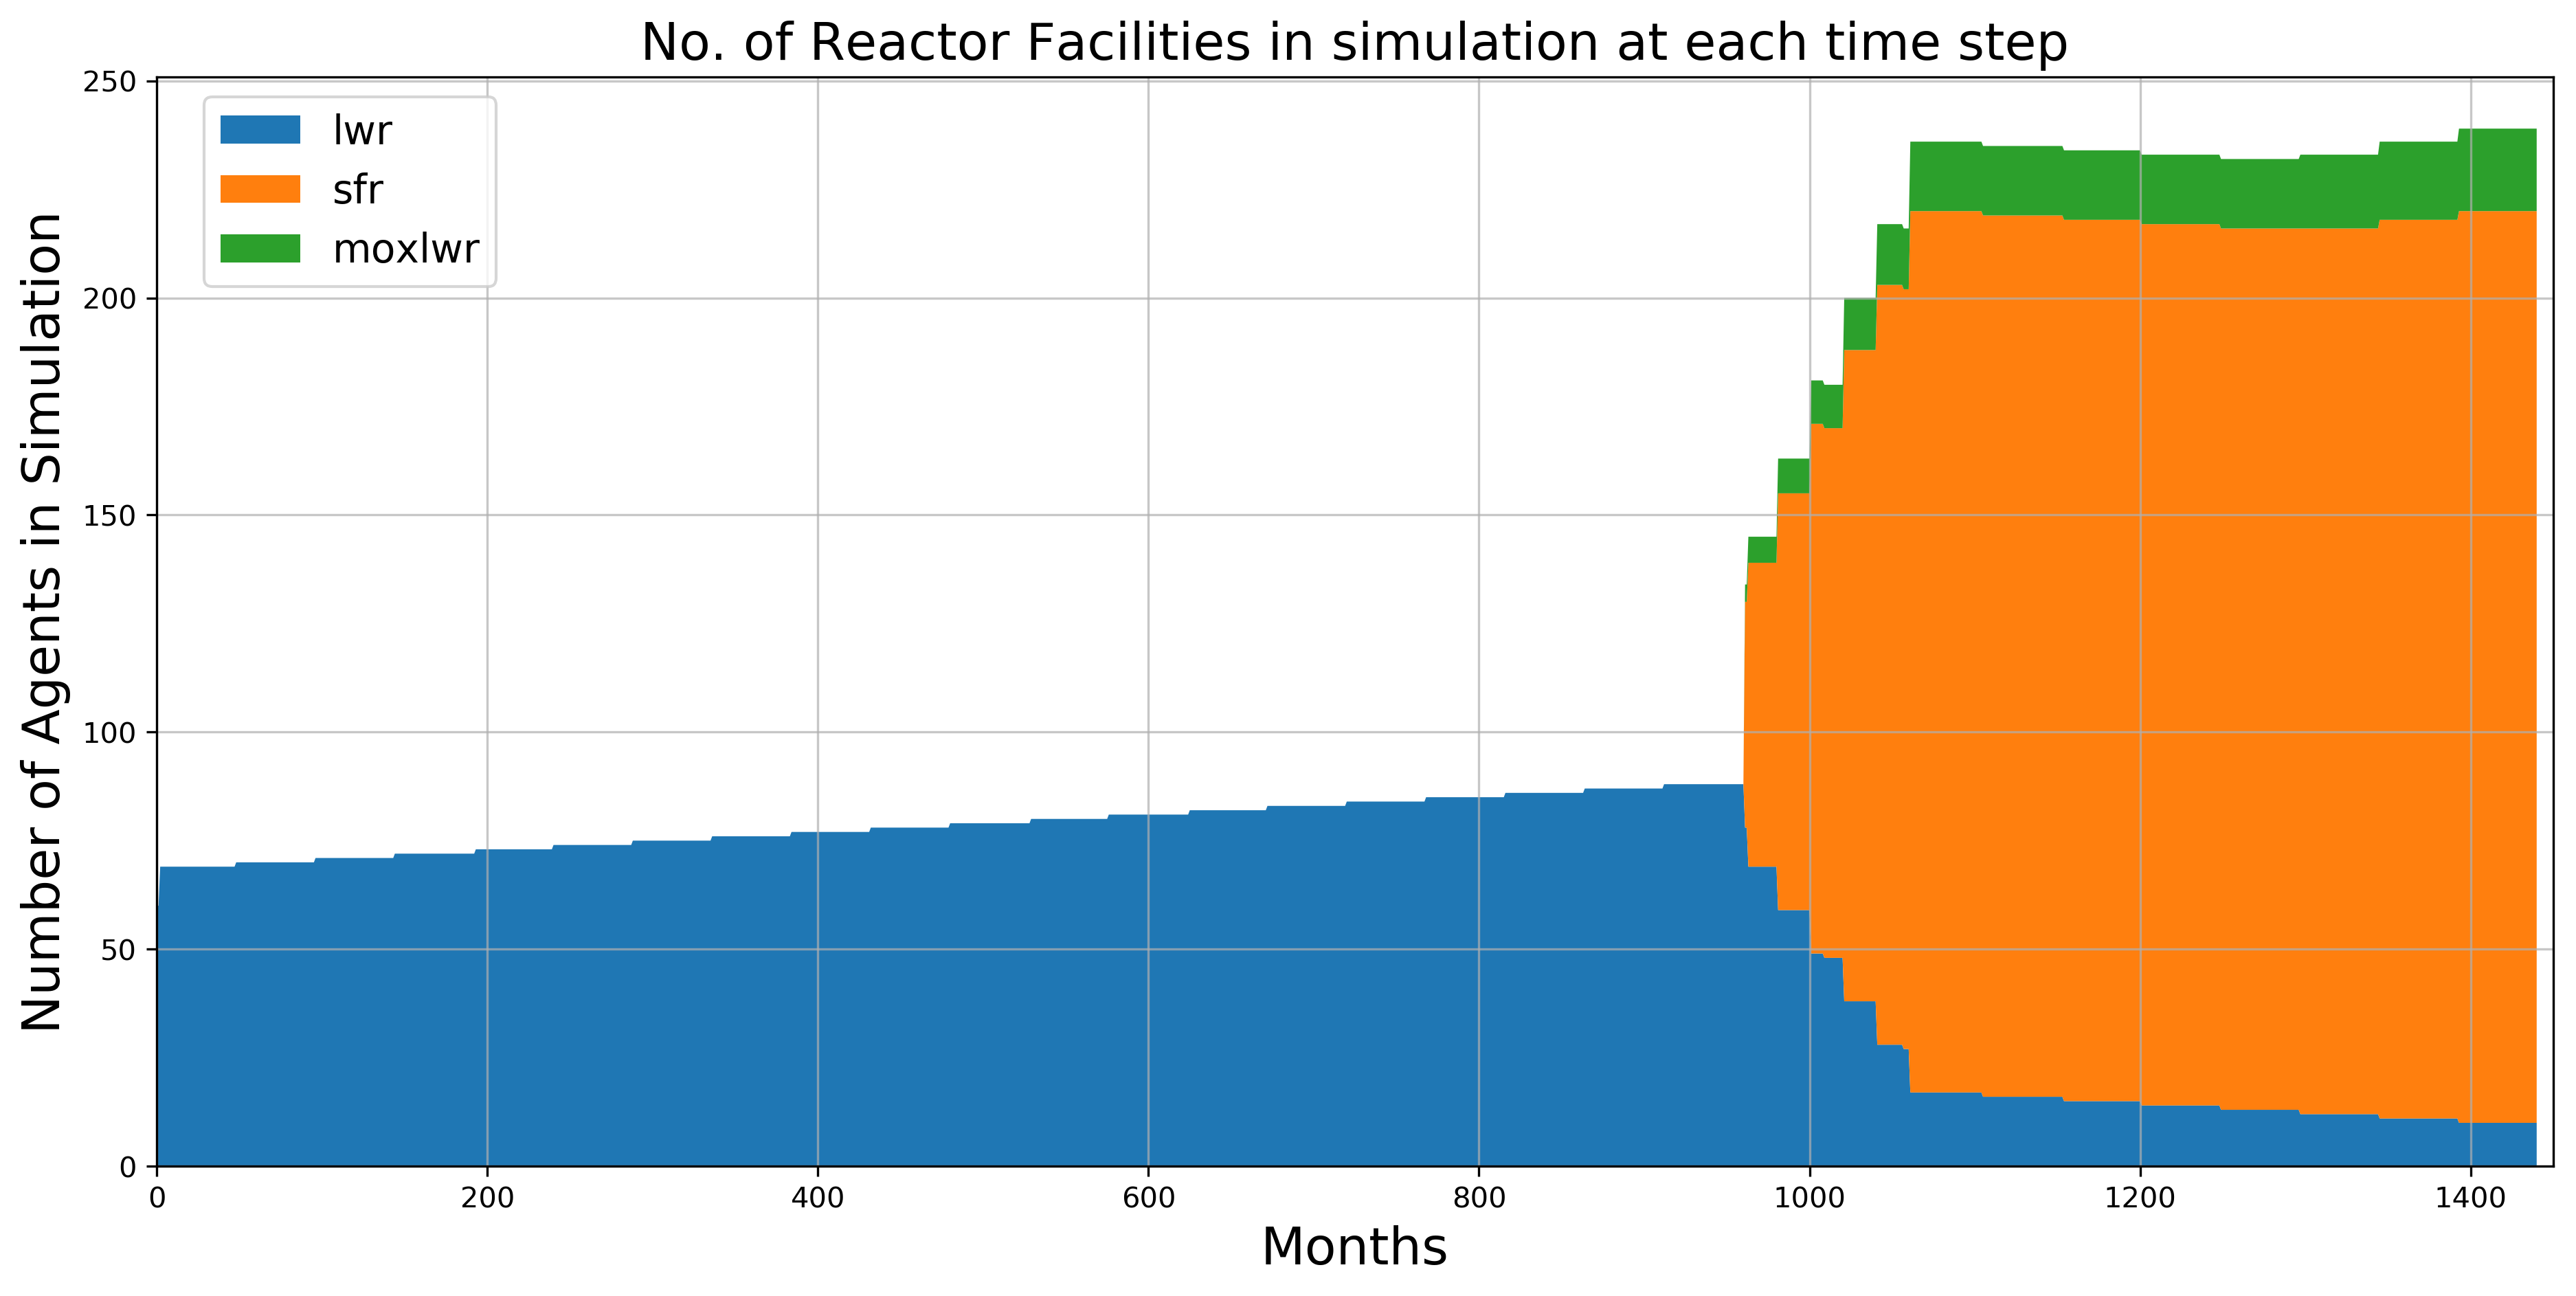
\includegraphics[width=\linewidth]{eg30-stack_reactor.png} 
            \caption{EG01-30: Reactor Deployment}
            \label{fig:30reactor}
        \end{subfigure}
        \vspace{1cm}
        \begin{subfigure}[t]{\textwidth}
            \centering
            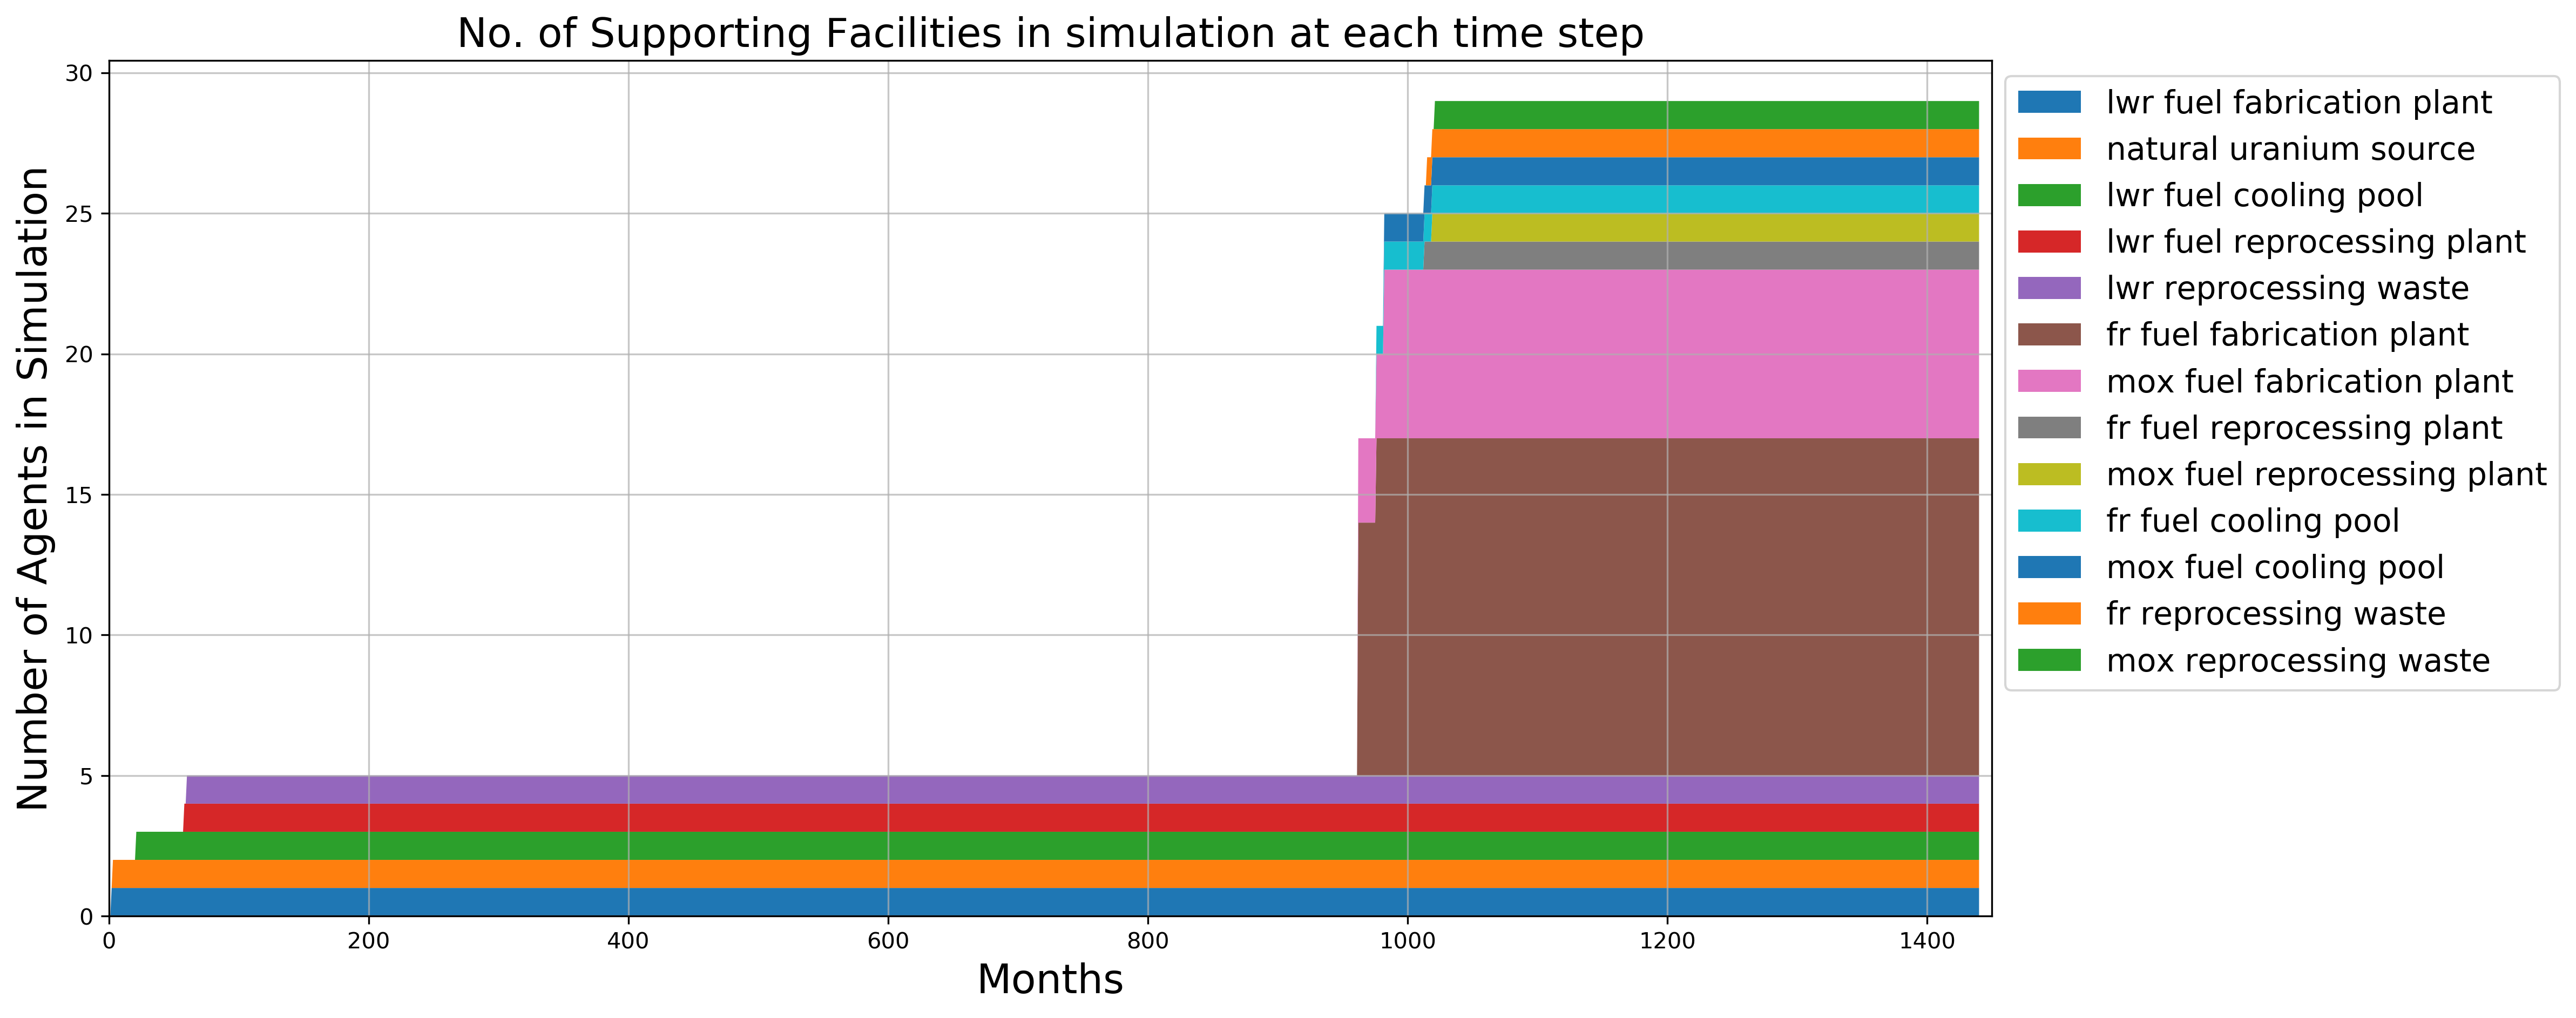
\includegraphics[width=\linewidth]{eg30-stack_support.png} 
            \caption{EG01-30: Supporting Facility Deployment}
            \label{fig:30support}
        \end{subfigure}
        \hfill
        \caption{Time dependent deployment of reactor and supporting facilities in 
        the EG01-30 linearly increasing power demand transition scenario. 
        \deploy automatically deploys reactor and supporting facilities 
        to setup a supply chain to meet linearly increasing power demand of $60000 + 250t/12$ MW
        during a transition from \glspl{LWR} to MOX LWRs and \glspl{SFR}. }
        \label{fig:30stack}
    \end{figure}
